\documentclass[sigconf
%   anonymous,
%	timestamp,
]{acmart}
\pagestyle{plain}

\copyrightyear{2017} 
\acmYear{2017} 
\setcopyright{acmlicensed}
\acmConference{AISec'17}{November 3, 2017}{Dallas, TX, USA}
\acmPrice{15.00}
\acmDOI{10.1145/3128572.3140443}
\acmISBN{978-1-4503-5202-4/17/11}
\fancyhead{}

\settopmatter{printccs=false,printfolios=false}
%\renewcommand\footnotetextcopyrightpermission[1]{} % removes footnote with conference information in first column

\usepackage{booktabs} % For formal tables
\usepackage{tikz}
\usepackage{multirow}
\usepackage{amssymb}
\usepackage{url}
\usepackage{amsfonts}
\usepackage{amsmath}
\usepackage{pifont}
\usepackage{enumitem}
\usepackage{hyperref}
\usepackage{tabulary}
\usepackage{mathabx}
\usepackage{stmaryrd}
\usepackage{xspace}
\usepackage{graphicx}
\usepackage[export]{adjustbox}
\usepackage{multirow}
\usepackage{subcaption}
\usepackage{listings}
\usepackage{color, colortbl}

\definecolor{Gray}{gray}{0.9}

\newcommand*\rot{\rotatebox{65}}
\newcommand{\saumya}{\textcolor{black}{\ding{51}}}
\newcommand{\xmark}{\textcolor{red}{\ding{55}}}
\newcommand{\note}[1]{\textbf{\textcolor{blue}{[#1]}}}
\newcommand\jason[1]{%
	\textcolor{red}{[\textbf{}
	\ignorespaces #1%
	\ifhmode
		\unskip
	\fi
	]}%
}

\newcommand{\re}{ReCaptcha\xspace}
\newcommand{\system}{AudioBreaker\xspace}
\newcommand{\no}{seven\xspace}

\setlist{leftmargin=2\parindent,
         labelindent=\parindent,
	 labelwidth=*,
	 labelsep*=.5em}

% Print a big black box next to any overfull hboxes.
%\overfullrule=5pt

%%%%%%%%command for circles with alphanumeric inside
\definecolor{azure}{RGB}{0,127,255}

\newcommand*\circlea[1]{\protect\tikz[baseline=(char.base)]{
\node[shape=circle, white, font=\sffamily\bfseries, draw=black,
fill=black,inner sep=2pt] (char) {#1};}}

\newcommand*\circleaa[1]{\protect\tikz[baseline=(char.base)]{
\node[shape=circle, white, font=\sffamily\bfseries, draw=black,
fill=black,inner sep=1pt] (char) {#1};}}

\newcommand*\circleb[1]{\protect\tikz[baseline=(char.base)]{
\node[shape=circle, white, font=\sffamily\bfseries, draw=red,
fill=red,inner sep=2pt] (char) {#1};}}

\newcommand*\circlebb[1]{\protect\tikz[baseline=(char.base)]{
\node[shape=circle, white, font=\sffamily\bfseries, draw=red,
fill=red,inner sep=1pt] (char) {#1};}}

\newcommand*\circlec[1]{\protect\tikz[baseline=(char.base)]{
\node[shape=circle, white, font=\sffamily\bfseries, draw=azure,
fill=azure,inner sep=2pt] (char) {#1};}}

%%%%%%%%%%%%%%%%%%json listings
\colorlet{punct}{red!60!black}
\definecolor{background}{HTML}{EEEEEE}
\definecolor{delim}{RGB}{20,105,176}
\colorlet{numb}{magenta!60!black}

\newcommand\JSONnumbervaluestyle{\color{blue}}
\newcommand\JSONstringvaluestyle{\color{red}}

\lstdefinelanguage{json}{
    basicstyle=\scriptsize\ttfamily,
    showstringspaces=false,
    keywords={transcript,confidence,alternatives,BotDetect,CaptchasNet},
    keywordstyle=\color{blue},
    breaklines=true,
    morestring = [s]{"}{"},
    stringstyle=\color{red},
    float=t,
    frame=single,
    breakatwhitespace=true,
    captionpos=b,
    comment=[l]{//},
    commentstyle=\itshape\color{green!40!black},
    morekeywords={IBM,Wit}
    %stringstyle=\color{green},
    backgroundcolor=\color{background},
    literate=
     *{0}{{{\color{numb}0}}}{1}
      {1}{{{\color{numb}1}}}{1}
      {2}{{{\color{numb}2}}}{1}
      {3}{{{\color{numb}3}}}{1}
      {4}{{{\color{numb}4}}}{1}
      {5}{{{\color{numb}5}}}{1}
      {6}{{{\color{numb}6}}}{1}
      {7}{{{\color{numb}7}}}{1}
      {8}{{{\color{numb}8}}}{1}
      {9}{{{\color{numb}9}}}{1}
      {:}{{{\color{punct}{:}}}}{1}
      {,}{{{\color{punct}{,}}}}{1}
      {\{}{{{\color{delim}{\{}}}}{1}
      {\}}{{{\color{delim}{\}}}}}{1}
      {[}{{{\color{delim}{[}}}}{1}
      {]}{{{\color{delim}{]}}}}{1},
}
%%%%%%%%

%% Copyright
%%\setcopyright{none}
%%\setcopyright{acmcopyright}
%%\setcopyright{acmlicensed}
%\setcopyright{rightsretained}
%%\setcopyright{usgov}
%%\setcopyright{usgovmixed}
%%\setcopyright{cagov}
%%\setcopyright{cagovmixed}
%
%
%% DOI
%\acmDOI{xxx}
%
%% ISBN
%\acmISBN{xxx}
%
%%Conference
%\acmConference[CCS'17]{ACM Symposium on Computer and Communication
%Security}{November 2017}{Dallas, TX, USA} 
%\acmYear{2017}
%\copyrightyear{2017}
%
%\acmPrice{00.00}
%
%\acmSubmissionID{xxx-xxx-xx}
%
%\title{In (Cyber)Space Bots Can Hear You: \\ Speech Recognition Attacks Against Audio CAPTCHAs}
%\title{In CyberSpace Bots Can Hear You (Scream): \\ Breaking Audio Captchas Using Speech Recognition}
\title{In (Cyber)Space Bots Can Hear You Speak: \\ Breaking Audio CAPTCHAs Using OTS Speech Recognition}

% We can actually set the authors now and remove the `anonymous` class option
% above for camera ready.
\author{Anonymous}
\begin{document}

% The new ACM template is dumb. The abstract needs to be defined before the
% \maketitle! See acmart.pdf.
\begin{abstract}

Captchas have become almost ubiquitous and are commonly deployed by websites as part of their 
defenses against fraudsters. However visual captchas pose a
considerable obstacle to certain groups of users, such as the visually impaired,
and that has necessitated the inclusion of more accessible captcha schemes.
As a result, many captcha services also offer audio challenges as an alternative.

In this paper we conduct an extensive exploration of the audio captcha ecosystem,
and present effective low-cost attacks against the audio challenges offered by seven major
captcha services. Motivated by the recent advancements in deep learning, we demonstrate
how off-the-shelf speech recognition services can be misused by fraudsters for trivially
bypassing the most popular audio captchas. Our experimental evaluation highlights the effectiveness 
of our approach as our \system system achieves a success rate of \note{X-Y\%}.
The broader implications of our study are twofold. First, we find that the wide availability of advanced
speech recognition services has severely lowered the technical capabilities required by fraudsters
for deploying effective attacks, as there is no longer a need for building sophisticated custom classifiers.
Second, we find that the availability of audio captchas poses a significant risk to services,
as we achieve a \note{x\%} higher attack accuracy against \re's audio challenges compared to 
recent state-of-the-art attacks against their image-based challenges. Overall, we argue that it 
is necessary to explore alternative captcha designs that fulfill the accessibility properties 
of audio captchas without undermining the security offered by their visual counterparts.

\end{abstract}

\keywords{Audio Captchas, Speech Recognition, Captcha Solving}
\maketitle

\section{Introduction}
\label{sec:intro}

While automated attacks continue to plague the Internet,
the number of of online users around the world has reached unprecedented levels.
Thus, it is crucial to deploy user-friendly mechanisms for preventing bots without
becoming obstacles to legitimate users. Traditionally captchas comprise the first 
line of defense, and attempt to differentiate between actual users and bots by 
presenting a challenge that requires some form of task that is considered hard 
for a computer~\cite{captcha}. While visual captchas (i.e., text and image based challenges) 
have evolved significantly since their initial incarnation, with Google's recent \re system 
attempting to bridge the gap between security and usability, audio captchas have remained 
relatively unchanged.

Audio captchas are deployed as an alternative type of challenge, targeting
visually-impaired users that would otherwise not be able to pass the presented
challenge. According to the World Health Organization 285 million people have 
some form of visual impairment~\cite{impaired}, rendering audio captchas a
crucial component of an inclusive world wide web. While audio captchas may still present
an obstacle to certain users~\cite{sauer2008towards,bigham2008inspiring,bigham2009evaluating},
they are currently the de facto alternative offered by captcha services.

While audio captchas have not received as much attention from the security community as visual captchas,
previous work has presented automated attacks against audio captchas~\cite{Sano2013,Bursztein2009,
meutzner2014using,tam2009breaking,bursztein2011failure}. These studies have demonstrated attacks
that achieve high accuracy by building customs classifiers using machine learning techniques.
However, the tremendous advancements of the past years in deep learning technology, have
resulted in significant improvements in speech recognition systems, recently achieving
results that approach human performance~\cite{ibm_blog,saon2017english}. Motivated
by these advancements, and the recent work by Sivakorn et al. against visual
captchas~\cite{sivakorn:eurosp16}, we investigate how speech recognition services
can be misused for breaking existing audio captcha systems. By exploring how effective
widely-available speech recognition systems are at transcribing audio challenges despite 
the presence of noise, typically present in captcha challenges, we can assess the robustness 
of the captcha ecosystem.

In this work we present \system, a modular system that leverages existing speech recognition services
for solving audio captcha challenges. Specifically, we leverage the
APIs offered by IBM's Watson, Facebook's Wit, and Google's Cloud Speech. In a nutshell, our system works as
follows. First, our browser automation module visits a page protected by one of the captcha services,
and obtains the audio challenge. Next, after minimal preprocessing, the audio recording is submitted 
to one of the speech recognition services. Upon receiving the transcription from the service, we 
process the text based on the properties of the specific captcha service (e.g., transcribing to alphanumeric 
from NATO's phonetic alphabet) and prepare the response to the challenge. This is then handled by
the browser automation module that inputs the response and checks whether it was accepted by the captcha
service.

We evaluate \system again \no captcha systems, including popular services like Google \re,
Apple's and Microsoft's captchas. Our experiments demonstrate the effectiveness of our approach,
as we are able to (greatly) surpass the threshold commonly set in prior work for considering
a captcha system broken, with the highest accuracy achieved against \re -- the most prevalent 
captcha system.

Surprising findings: every single one broken. Accent matters. Higher accuracy than prior work. Much higher accuracy than
visual captchas. Old \re harder than new \re. 
Apart from facilitating visually-impaired users, audio captchas introduce an attack
surface that presents a significantly smaller obstacle to attackers compared to visual captchas.

\note{Important takeaways. Broader impact.}

Overall, the main contributions of our work are:

\begin{itemize}

\item We present the first, to our knowledge, comprehensive evaluation of 
the audio captcha ecosystem against low-cost 
%by demonstrating how available   services 
%can be broken using 
attacks using off-the-shelf speech recognition services.

\item We bla bla bla.

\item We bla bla bla.

\end{itemize}

\section{Background}
\label{sec:background}

Give more background information about captchasi and audio captchas.

Talk about threat model, and what \% accuracy previous work has
set as a threshold for considering a captcha system broken.

\section{System Overview}
\label{sec:system}

\begin{figure}
\centering
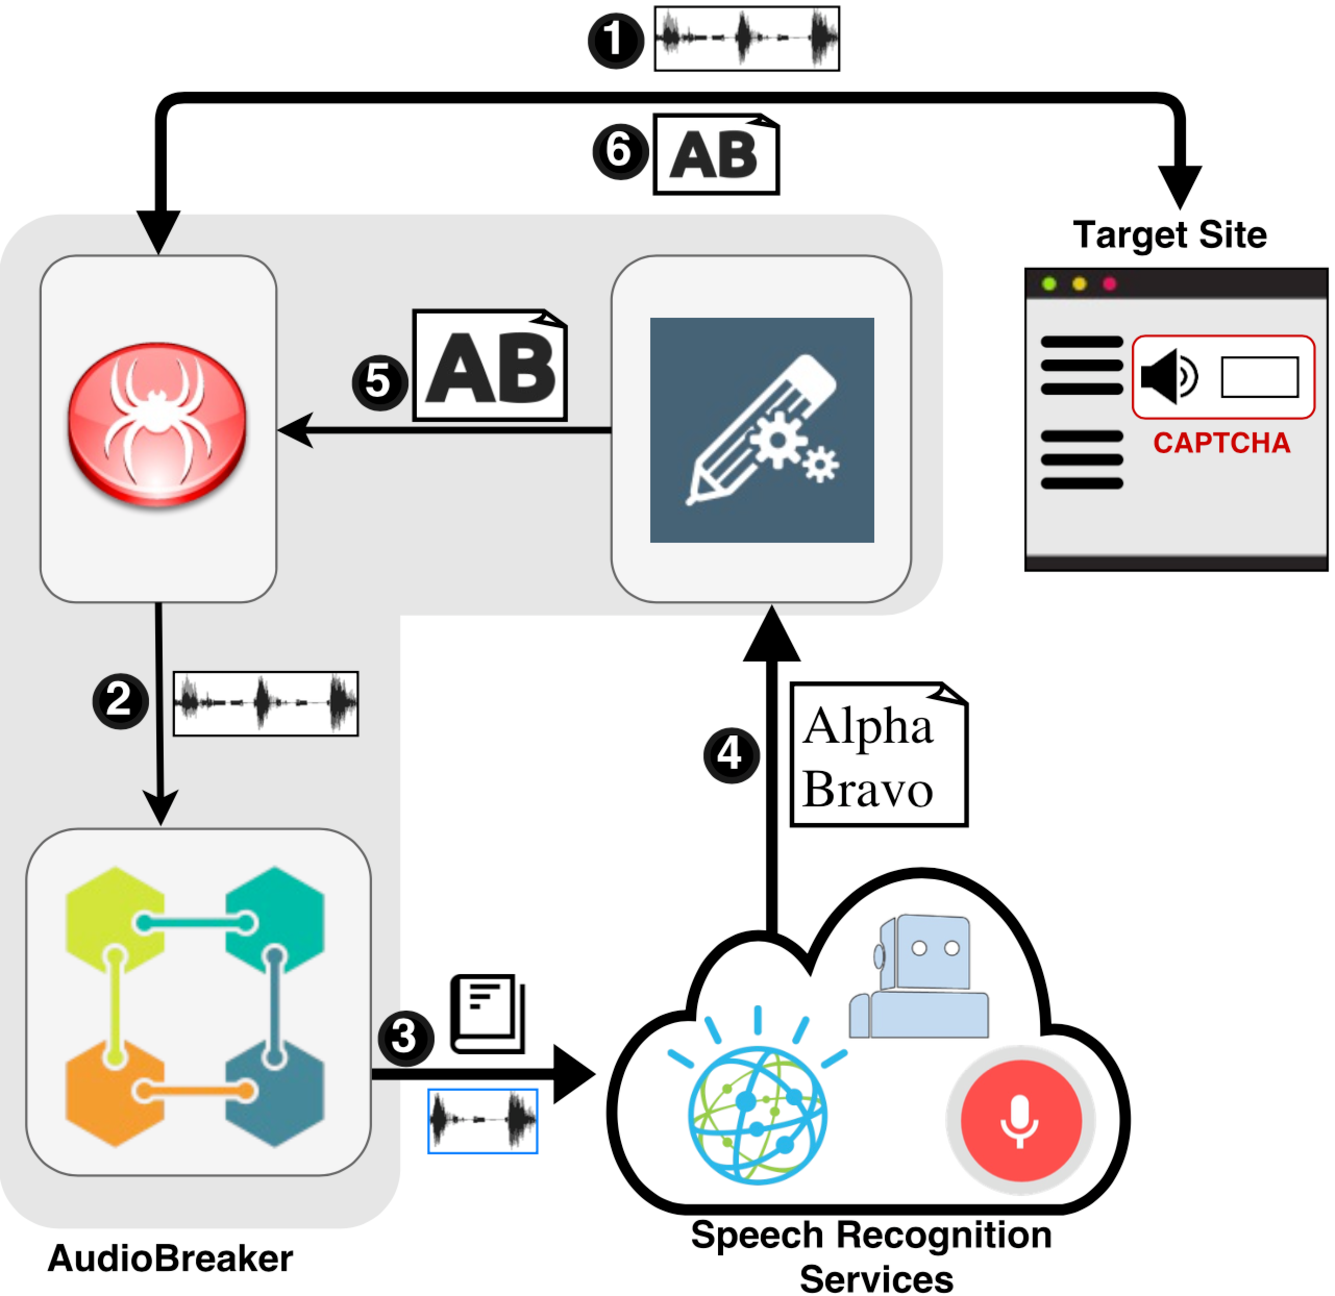
\includegraphics[width=\columnwidth]{figures/breaker_arch.pdf}
\caption{Overview of the \system system and the captcha-solving workflow..}
\label{fig:breaker}
\end{figure}

In this section we first present an overview of \system's design and describe the automated 
captcha-solving process. We then offer more details on our system's implementation.

\subsection{\system Design}

One of the main goals of our work is to explore the effectiveness of different speech recognition
services against a large number of different audio captcha services. To that end, we opted for 
a modular design for \system, as that provides flexibility in adding support for new captcha 
systems and speech recognition APIs. Our system is comprised of 3 basic components. The main 
component is responsible for the browser automation and handles all browser-related actions,
including crawling and rendering webpages, extracting the audio captchas, and providing the solutions
to the challenges. It also performs specific actions to mimic a user's steps and avoid triggering  
checks implemented by the captcha services for detecting bots (e.g., mouse over actions, or text 
box highlighting before solutions are input).
The second component completes some pre-processing and configuration steps 
necessary before the audio recordings are passed to the speech recognition services. The final 
component handles the post-processing of the transcribed text for preparing the solution that will
be submitted to the captcha service.

Figure~\ref{fig:breaker} presents the main components of \system and outlines the workflow of
an automated attack against a target website that protects a specific action with a captcha 
service that also supports audio challenges.

\protect\circlea{\small 1} Our system visits a webpage that offers the desired functionality 
(e.g., account creation, message posting, etc.). After identifying the captcha element within 
the page, the audio challenge is extracted.

\protect\circlea{\small 2} The audio file is passed to the pre-processing component, which is responsible 
for preparing the audio file that will be passed to the speech recognition service. If there are audio 
instructions at the beginning of the audio challenge they are removed, and the final audio
recording is then converted to a lossless format. Then, based on the captcha service, our system
selects the speech recognition service with the best results for the specific challenge.

\protect\circlea{\small 3} The audio file is uploaded for "transcript"ion by the module that handles that solver, 
together with a predetermined configuration. The configuration allows us to fine-tune the "transcript"ion process
for better results; specifically we restrict the dictionary used by the solver (e.g., to only expect  
numbers) as well as the accent classifier to use (services may support multiple English accents 
-- British, American etc.).

\protect\circlea{\small 4} The ``transcription'' of the audio challenge is obtained from the solver 
and passed to the post-processing component. Based on the originating captcha service, the corresponding  
module will process the "transcript"ion and prepare the solution to the challenge. If a service employs the 
NATO phonetic alphabet, the transcribed words will be mapped to the letters they represent. For instance, 
``Alpha Bravo'' will be substituted with ``AB''. Furthermore, we have created manually curated dictionaries
per captcha service and speech recognition engine for further processing the "transcript"ions. This processing
also handles cases of homophones; for instance, $\{two,too,to\}$ are all
mapped to $\{2\}$ for captcha services that only contain digits in the audio challenges.

\protect\circlea{\small 5} The final solution is passed to the browser automation module,
which is responsible for passing the captcha challenge.

\protect\circlea{\small 6} The browser automation module inputs the solution while mimicking 
user behavior, as certain captcha services have deployed extra checks for identifying bots.
It also verifies whether the solution was accepted by the captcha service.

\subsection{Implementation Details}

\textbf{Browser automation.}
Our browser automation components is built upon the Selenium framework~\cite{selenium}. This offers
flexibility in setting up our environment (e.g., browser), as well as advanced functionality
and configurability that allow us to implement scraping behavior that does not trigger bot detection
mechanisms currently deployed by certain services\footnote{There is no straightforward way to detect 
automation apart for checking some predefined variables (which can be easily modified).}
%Most websites do not check these in practice.}.
Selenium communicates with the browser via a special protocol 
native to each browser, and has access to everything loaded for the visited web site, including all Javascript, DOM 
elements and even ``Secure'' HTTP cookies. The special protocol is required for communication with the browser,
and enables execution of the automation scripts without violating the same origin policy.
%In more detail, a sandbox is created for
%every website the browser creates a sandbox for the website's javascript, this way the javascript that 
%belongs to one website does not execute on another website that is currently loaded on the browser. 
%(more detail on cross site scripting). To overcome this 
Specifically, Selenium acts as an HTTP Proxy server when
the browser is launched through Selenium scripts, and Javascript (Selenium Core) is injected into the browser;
all subsequents requests are then handled through Selenium. In essence, the browser perceives the
web page as being served from Selenium's domain rather than the actual web server hosting the website.
As such, the automation scripts appear to belong to the same origin with the web page. This approach, 
however, faces certain limitations, which are handled by ``WebDriver'' an object oriented API
%as the Core is limited by the JavaScript sandbox of 
%the browser (Due to same origin policy). The Webdriver, 
which handles the browser from outside. 
%This was 
%the marked difference between Selenium 1.0 and Selenium 2.0 as by being limited by the sandbox and therefore 
%has reduced functional test coverage. 


\note{how do you automatically identify the captcha service being used on a random page?}

\textbf{Speech recognition APIs.}
We used three different voice recognition services for our system: Google's Cloud Speech API,
IBM Watsons Text-to-Speech API, and Facebook's Wit.ai voice recognition service. Below we 
provide some details regarding these services.

\begin{lstlisting}[language=json,firstnumber=1,caption={Example response from IBM Watson's API for an audio challenge from Google \re v2.a.},label={lst:IBM}]
{
results: [
{alternatives: [{transcript:"eight", confidence:0.982679}]},
{alternatives: [{transcript:"three", confidence:0.742102}]},
{alternatives: [{transcript:"eight", confidence:0.593190}]},
{alternatives: [{transcript:"nine", confidence:0.6004673}]},
{alternatives: [{transcript:"five", confidence:0.982679}]}
]
}

\end{lstlisting}

\emph{IBM Bluemix (Watson).} IBM Watson's Speech To Text service provides a public REST API, and the website provides 
sample code in multiple programming languages to facilitate integration.
%in Curl, Ruby and Node.JS with best practices for using their REST API. The API is also very well documented.
Their service accepts various audio file formats as input, and returns a 
with the timestamps of each recognized word, a confidence score, and alternative an hypothesis (if there is 
another interpretation for the word). It provides support for various languages 
like Spanish, Brazilian, Mandarin, Arabic, and two different accents in English - British and American.
%is available for free for the first 1000 min/per month for each 
%account, after which each additional minute is charged \$0.02. We used multiple accounts each to access the free 
%version of the software for the term of our project.

\emph{Wit.} Wit, which was acquired by Facebook in 2015, offers an API that leverages their natural language processing
capabilities and is geared towards developers building voice-activated interfaces (e.g., for home automation). We transform 
audio files to a WAV format (if required) in a monophonic (\emph{mono}) form as Wit does not currently support stereo format.
We use the ``free-text'' and ``keywords'' search strategies, that allow us \note{to identify values belonging to a predefined 
list of keywords}.

\emph{Google Cloud Speech.}  Google has released a RESTful API that offers access to a speech recognition system built on 
a deep learning neural network that can identify speech in over 80 languages. The API endpoint for recognizing speech supports
the ``phrases'' optional argument that allows us to narrow down the keywords their classifier model tries to identify, which 
results in higher accuracy against captcha schemes that use limited/restricted vocabularies (e.g., only digits). The Google
speech API also requires a mono form, and supports both WAV and FLAC file formats.

\begin{lstlisting}[language=json,firstnumber=1,mathescape=true,caption={Subset of rules use by our post-processing component for
converting keywords in transcription to elements of captcha's solution.},label={lst:rules}]
[BotDetect, *]: {hey,hay} $\longmapsto$ "a"
[BotDetect, IBM]: {three,through,tree,free,he,very,green} $\longmapsto$ "3"
[BotDetect, Wit;IBM]: {bee,be} $\longmapsto$ "b"
[CaptchasNet, Wit]: {gulf} $\longmapsto$ "golf"
[CaptchasNet, Wit]: {elsa} $\longmapsto$ "alpha"
\end{lstlisting}


\textbf{Post-processing.} Our post-processing component relies on a set of manually created rules that define transformations
of the transcribed audio to the string that will eventually be provided by our main component as the answer to the audio challenge.
These rules were created after extensive manual experimentation with each speech recognition service for each captcha scheme.
By identifying mis-identified words that are homonyms or sound somewhat similar to keywords that belong to the 
restricted dictionary of each captcha scheme (apart from Microsoft Live that uses common English words). This was motivated
by our observation of recurring mistakes that were made by each speech recognition service (some of which were common across
all three engines), which can be attributed to the ``consistent'' type of distortion and noise in each captcha system.
In Listing~\ref{lst:rules} we provide a few examples of our transformation rules.


\section{Audio Captcha Services}
\label{sec:services}

In this section we provide an overview of the captcha services that we found in the wild
that also provide audio captchas. We provide information on the characteristics of the audio challenges, as
well as some details about extra steps needed to avoid safeguards deployed by certain services for 
detecting automated attacks. Figure~\ref{fig:re_examples} and Figure~\ref{fig:examples} depict the waveform
and spectogram of sample challenges from each captcha service, allowing for a visual comparison
of the amount of background noise employed by each service.

%\jason{What are the checks deployed by each service? How do we bypass them? E.g., highlighting boxes etc.}

\begin{table}[t]
\centering
\caption{Description and characteristics of the captcha services that we evaluate.}
\begin{tabular}{lccc}
\toprule
\textbf{Service}& \textbf{Dictionary}& \textbf{Length} & \textbf{Noise} \\
\hline
%Recaptcha v1 & Digits & \jason{?} & None \\
Recaptcha v2.0 & Digits & 5 & None \\
\rowcolor{Gray}
Recaptcha v2.1 & Digits & 10 & None \\
Apple & Numbers (10-99) & 3-5 & Moderate\\
\rowcolor{Gray}
BotDetect & Digits, Alphabet & 1-13 & High \\
Captchas.net & NATO alphabet & 6 & None \\
\rowcolor{Gray}
Microsoft Live & Words & 5-7 & Moderate \\
Securimage & Digits, Alphabet & 6 & High \\
\rowcolor{Gray}
Telerik & Digits, NATO & 5 & None \\
\bottomrule
\end{tabular}
\label{tab:services}
\end{table}

\begin{figure}[tp]
%\begin{subfigure}{0.3\textwidth}
%        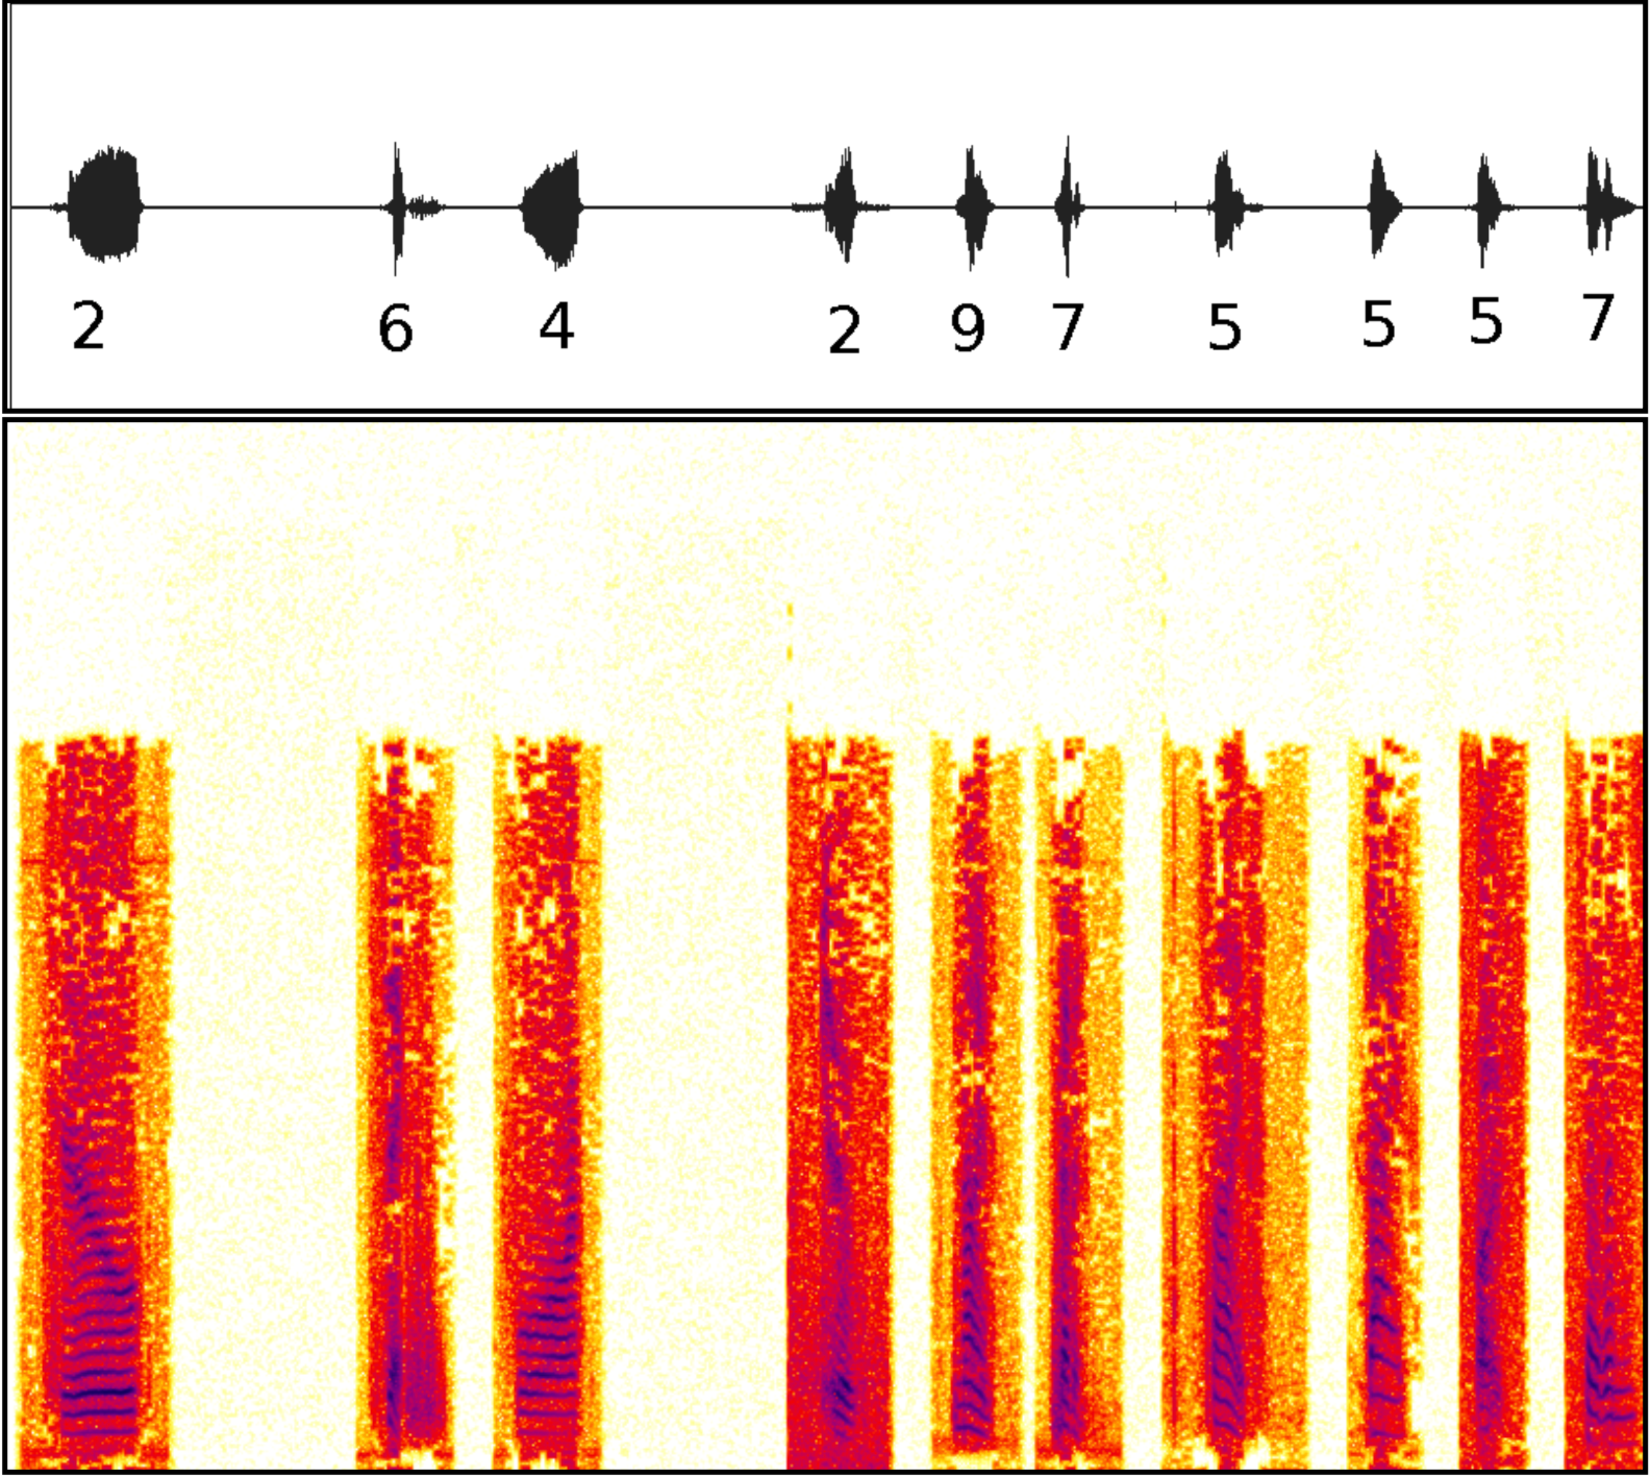
\includegraphics[width=\textwidth]{figures/recaptcha1.pdf}
%        \caption{\re v1}
%        \label{fig:recaptcha1}
%\end{subfigure} %\hspace{0.03\textwidth}
\begin{subfigure}{0.23\textwidth}
        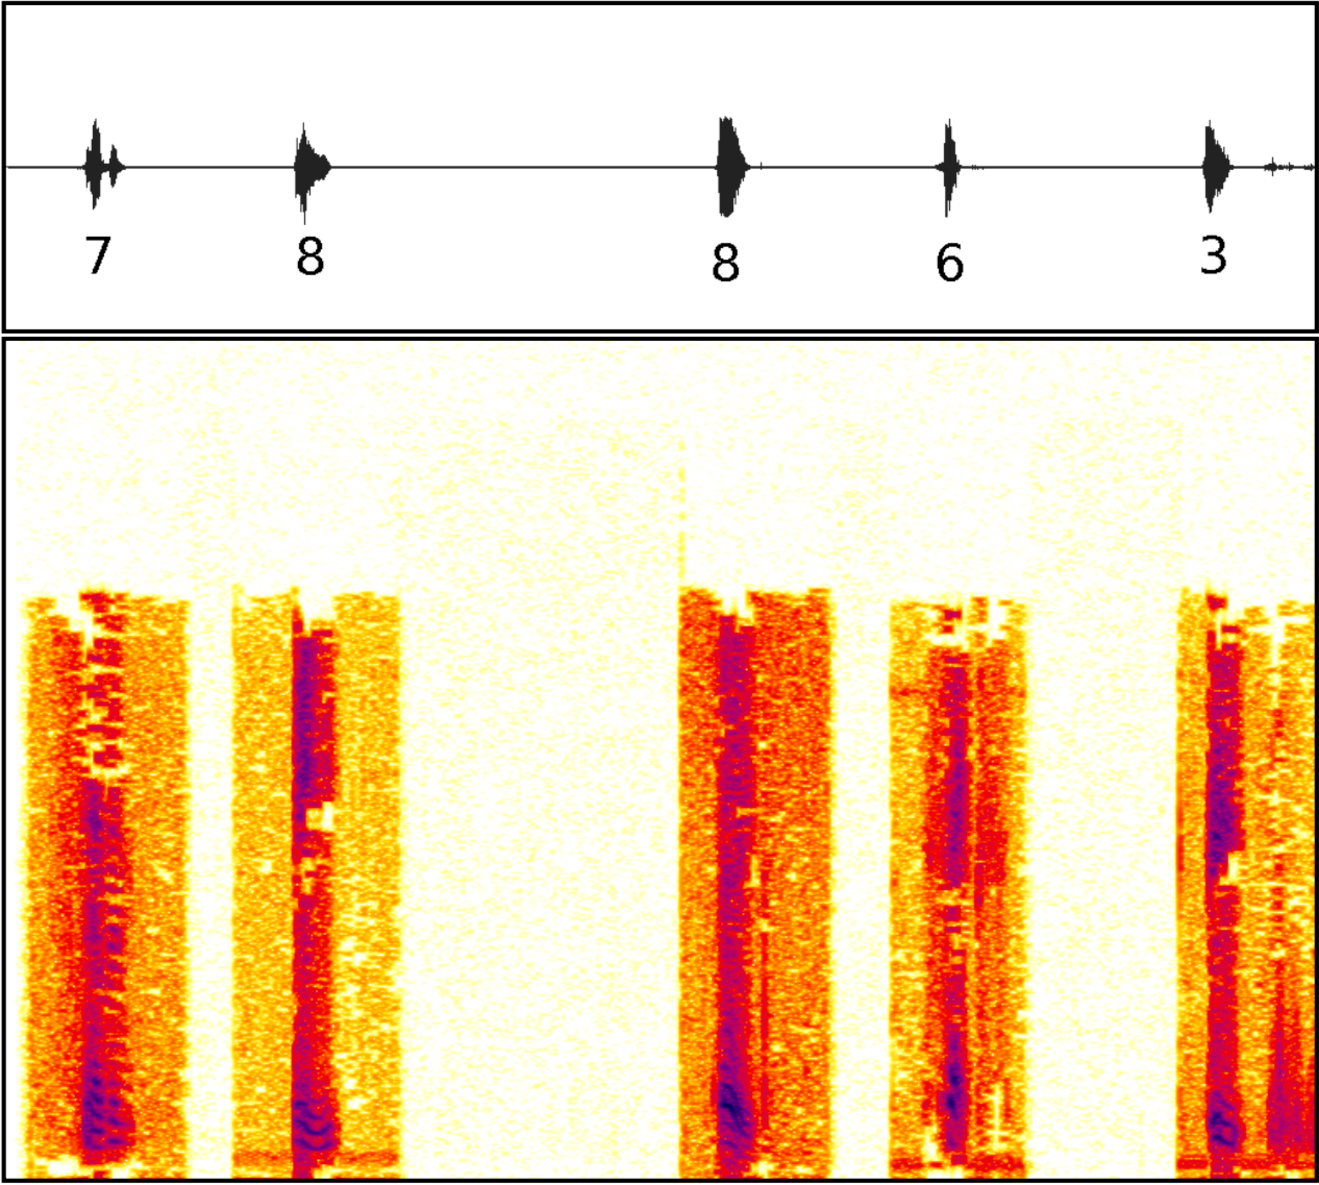
\includegraphics[width=\textwidth]{figures/recaptcha2a.pdf}
        \caption{\re v2.0}
        \label{fig:recaptcha2a}
\end{subfigure}\hspace{0.01\textwidth}
\begin{subfigure}{0.23\textwidth}
        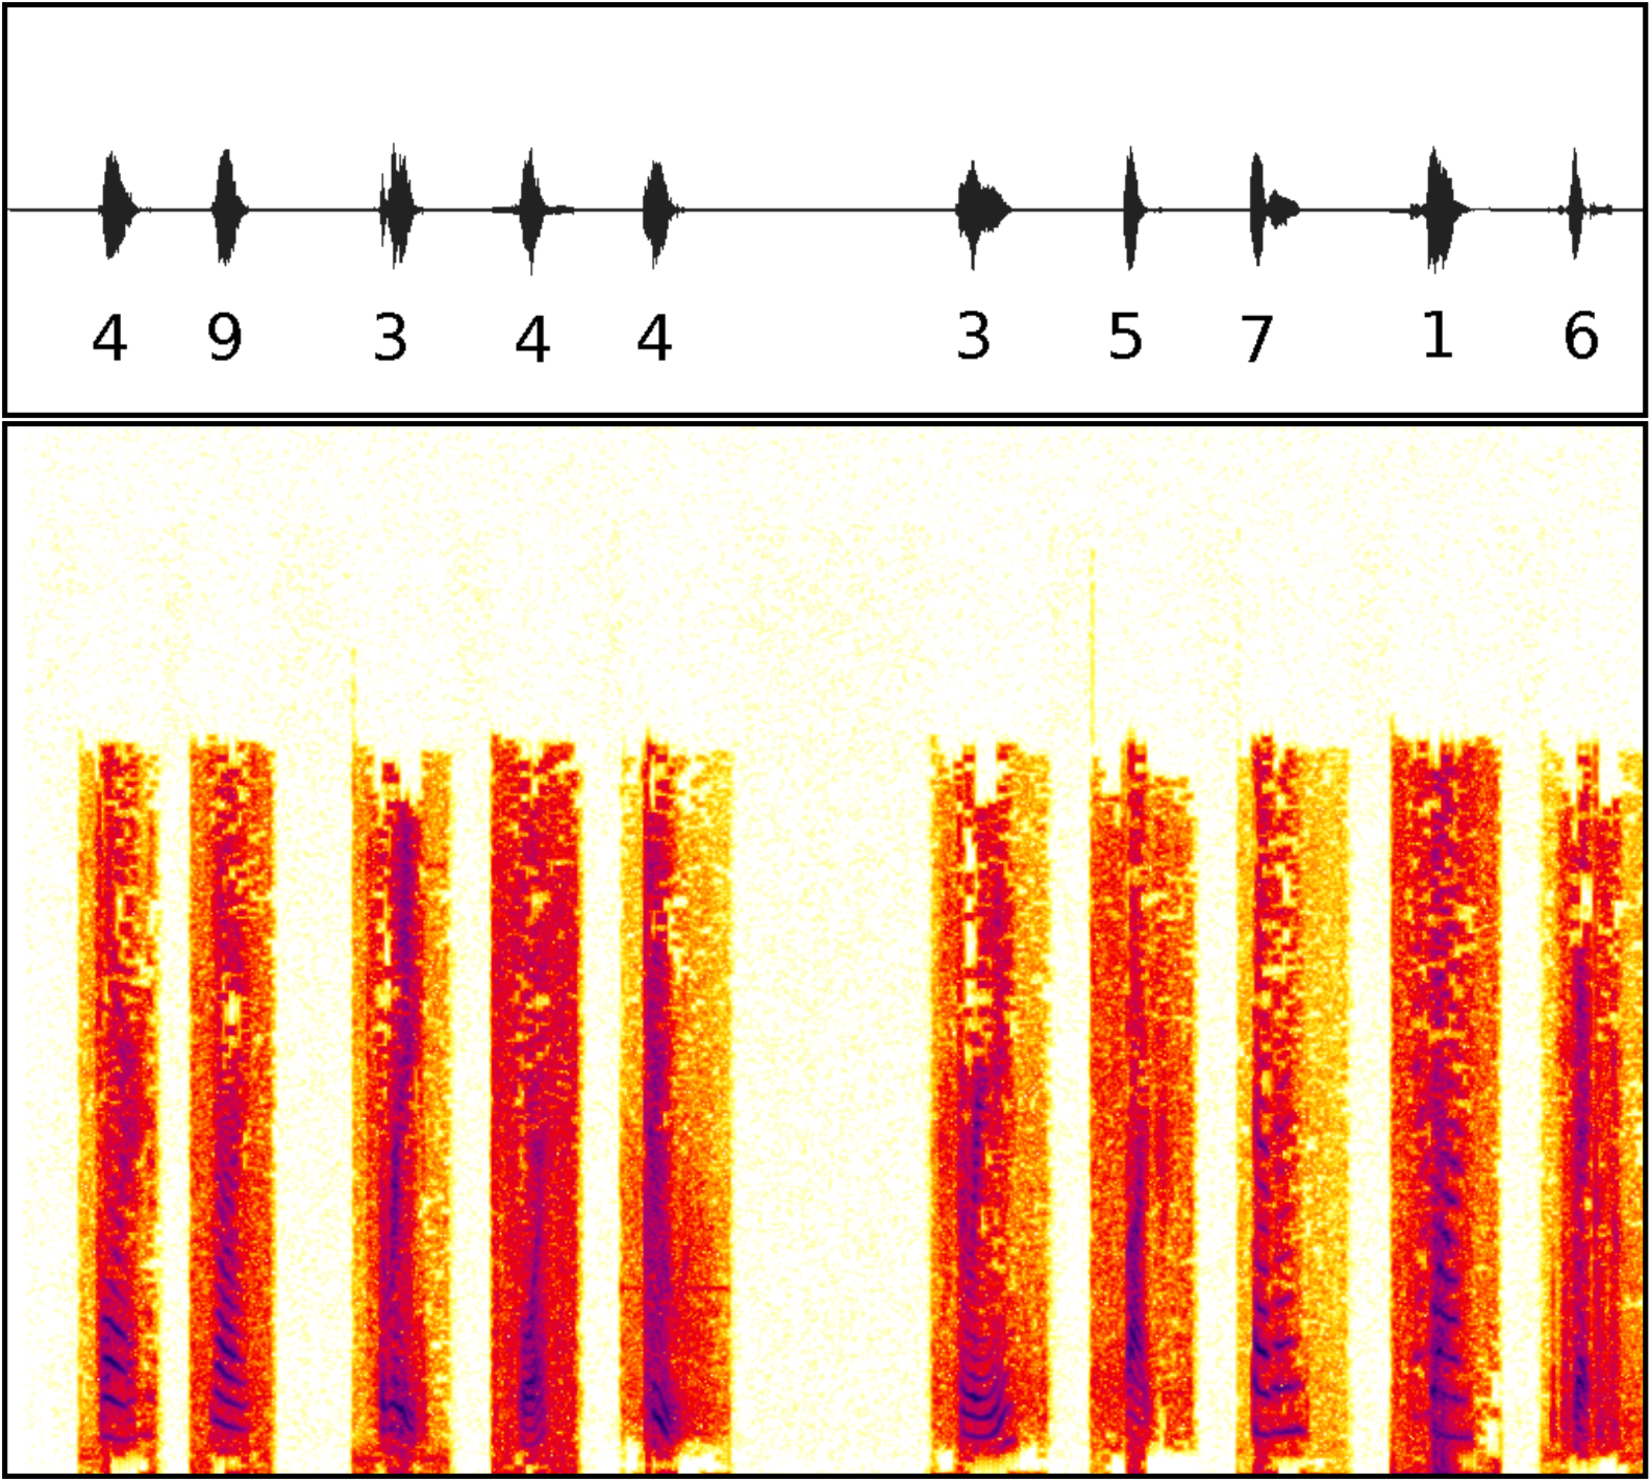
\includegraphics[width=\textwidth]{figures/recaptcha2b.pdf}
        \caption{\re v2.1}
        \label{fig:recaptcha2b}
\end{subfigure}
\caption{Waveforms and corresponding spectrograms for a representative sample challenge from the different versions of Google \re.}
\label{fig:re_examples}
\end{figure}

\begin{figure*}[tp]
\begin{subfigure}{0.3\textwidth}
        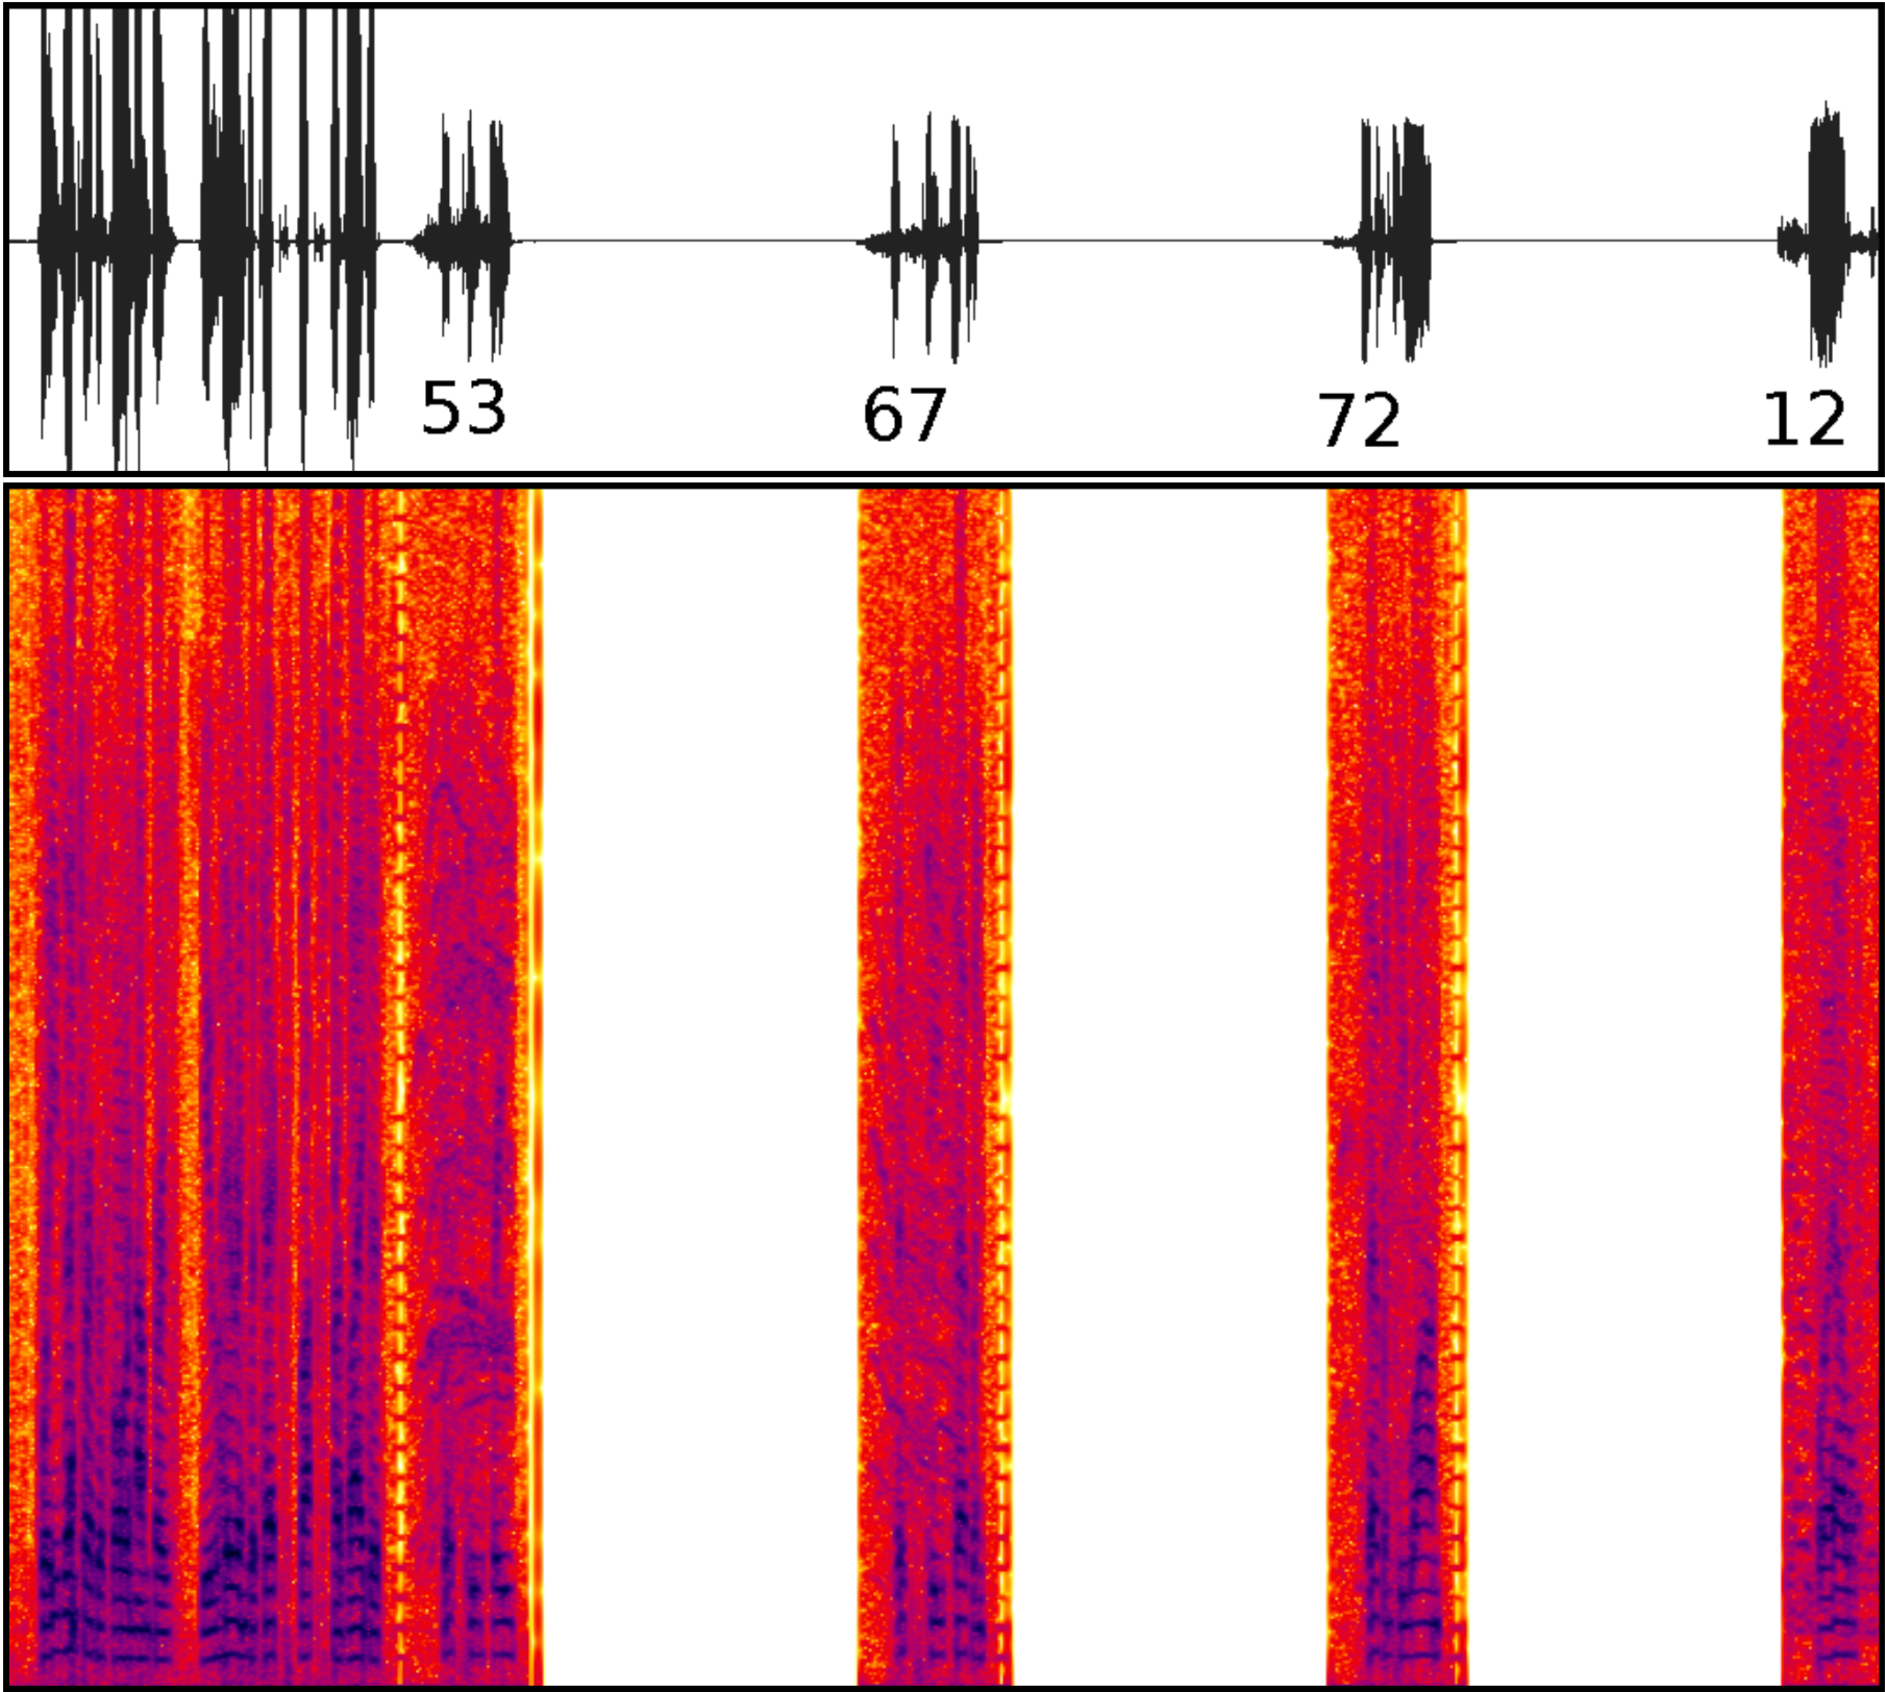
\includegraphics[width=\textwidth]{figures/apple.pdf}
        \caption{Apple}
        \label{fig:apple}
\end{subfigure} \hspace{0.03\textwidth}
\begin{subfigure}{0.3\textwidth}
        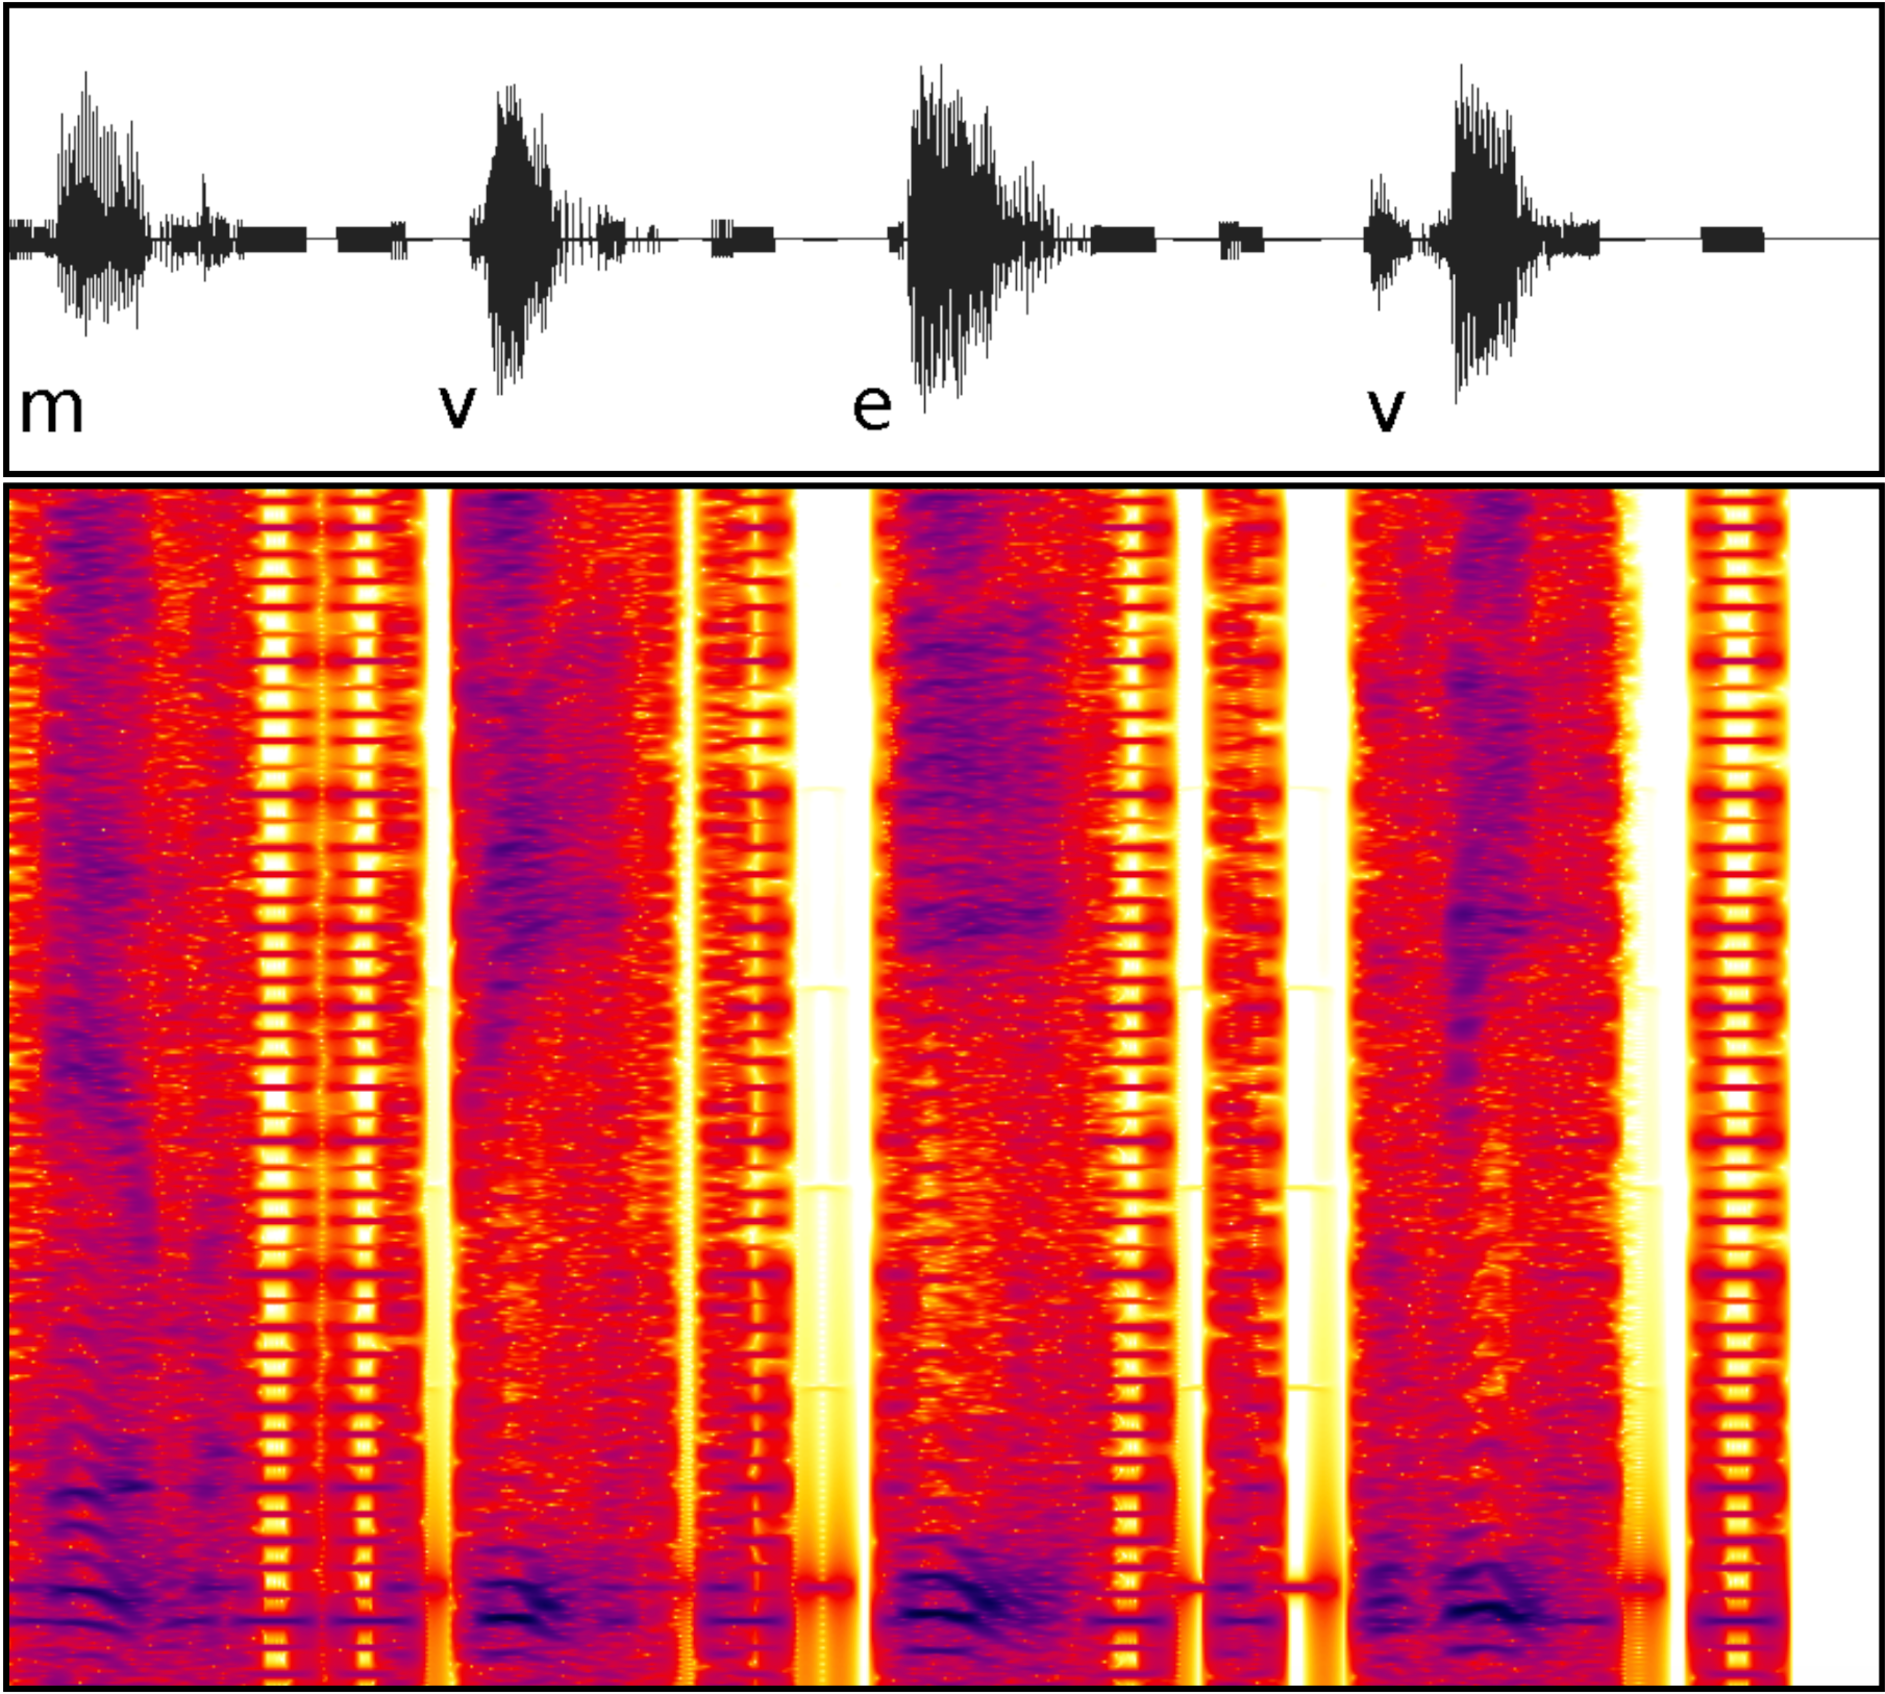
\includegraphics[width=\textwidth]{figures/botdetect.pdf}
        \caption{BotDetect}
        \label{fig:botdetect}
\end{subfigure}\hspace{0.03\textwidth}
\begin{subfigure}{0.3\textwidth}
        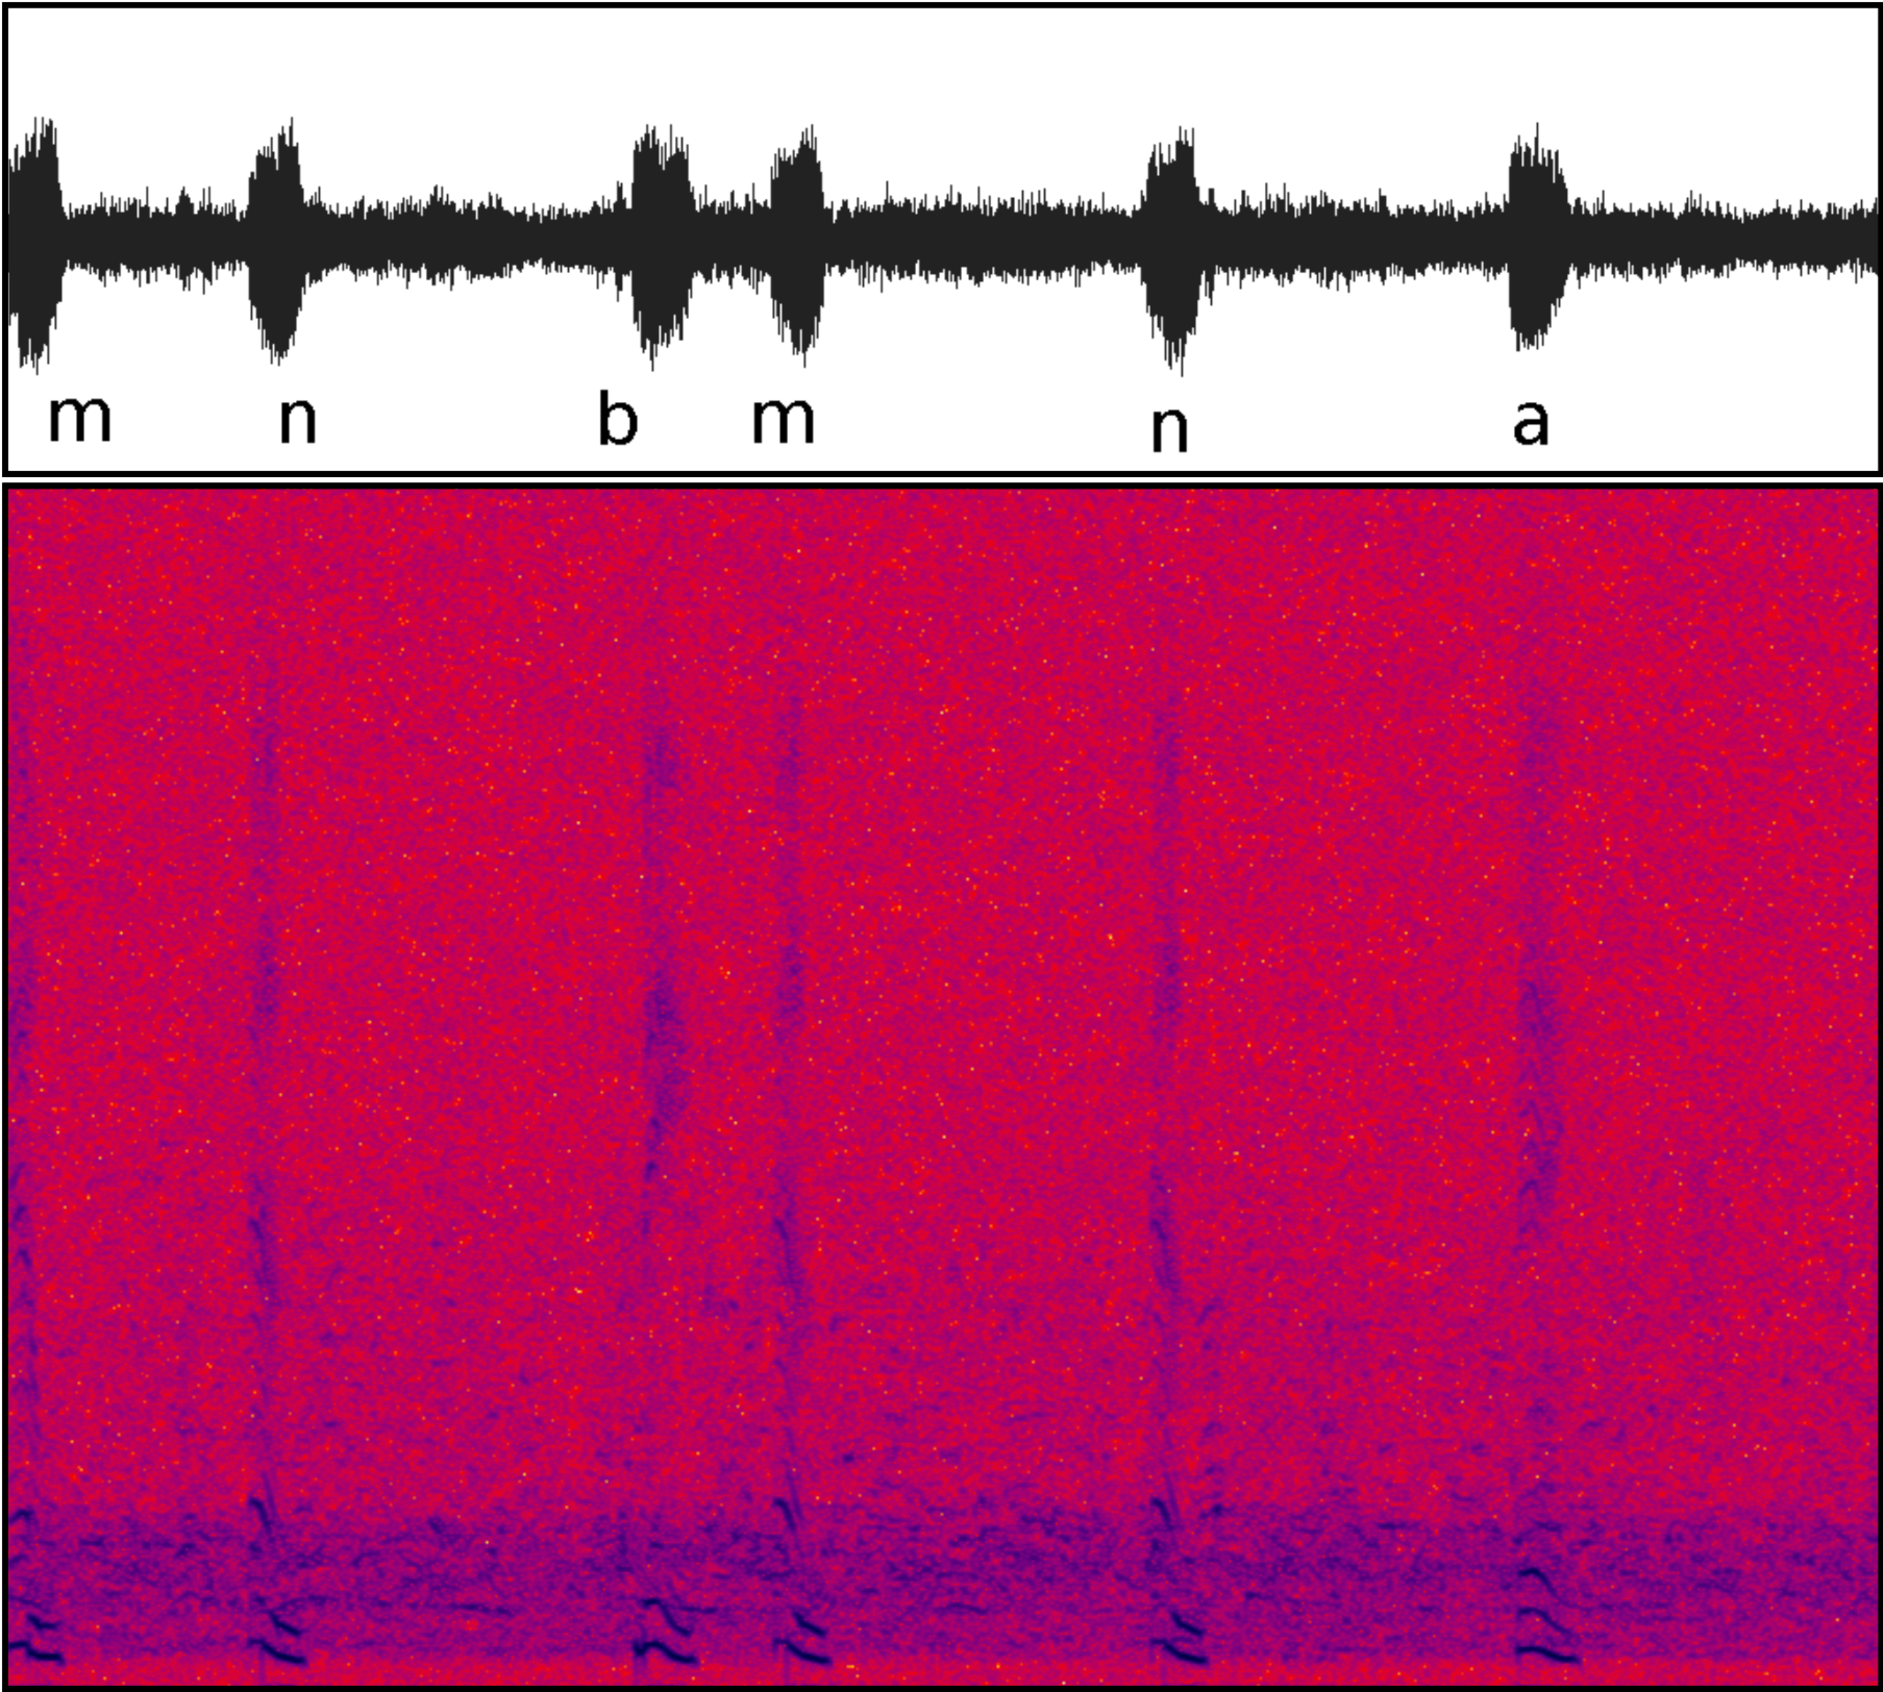
\includegraphics[width=\textwidth]{figures/captchas.pdf}
        \caption{Captchas.net}
        \label{fig:captchas}
\end{subfigure} \\
\begin{subfigure}{0.3\textwidth}
        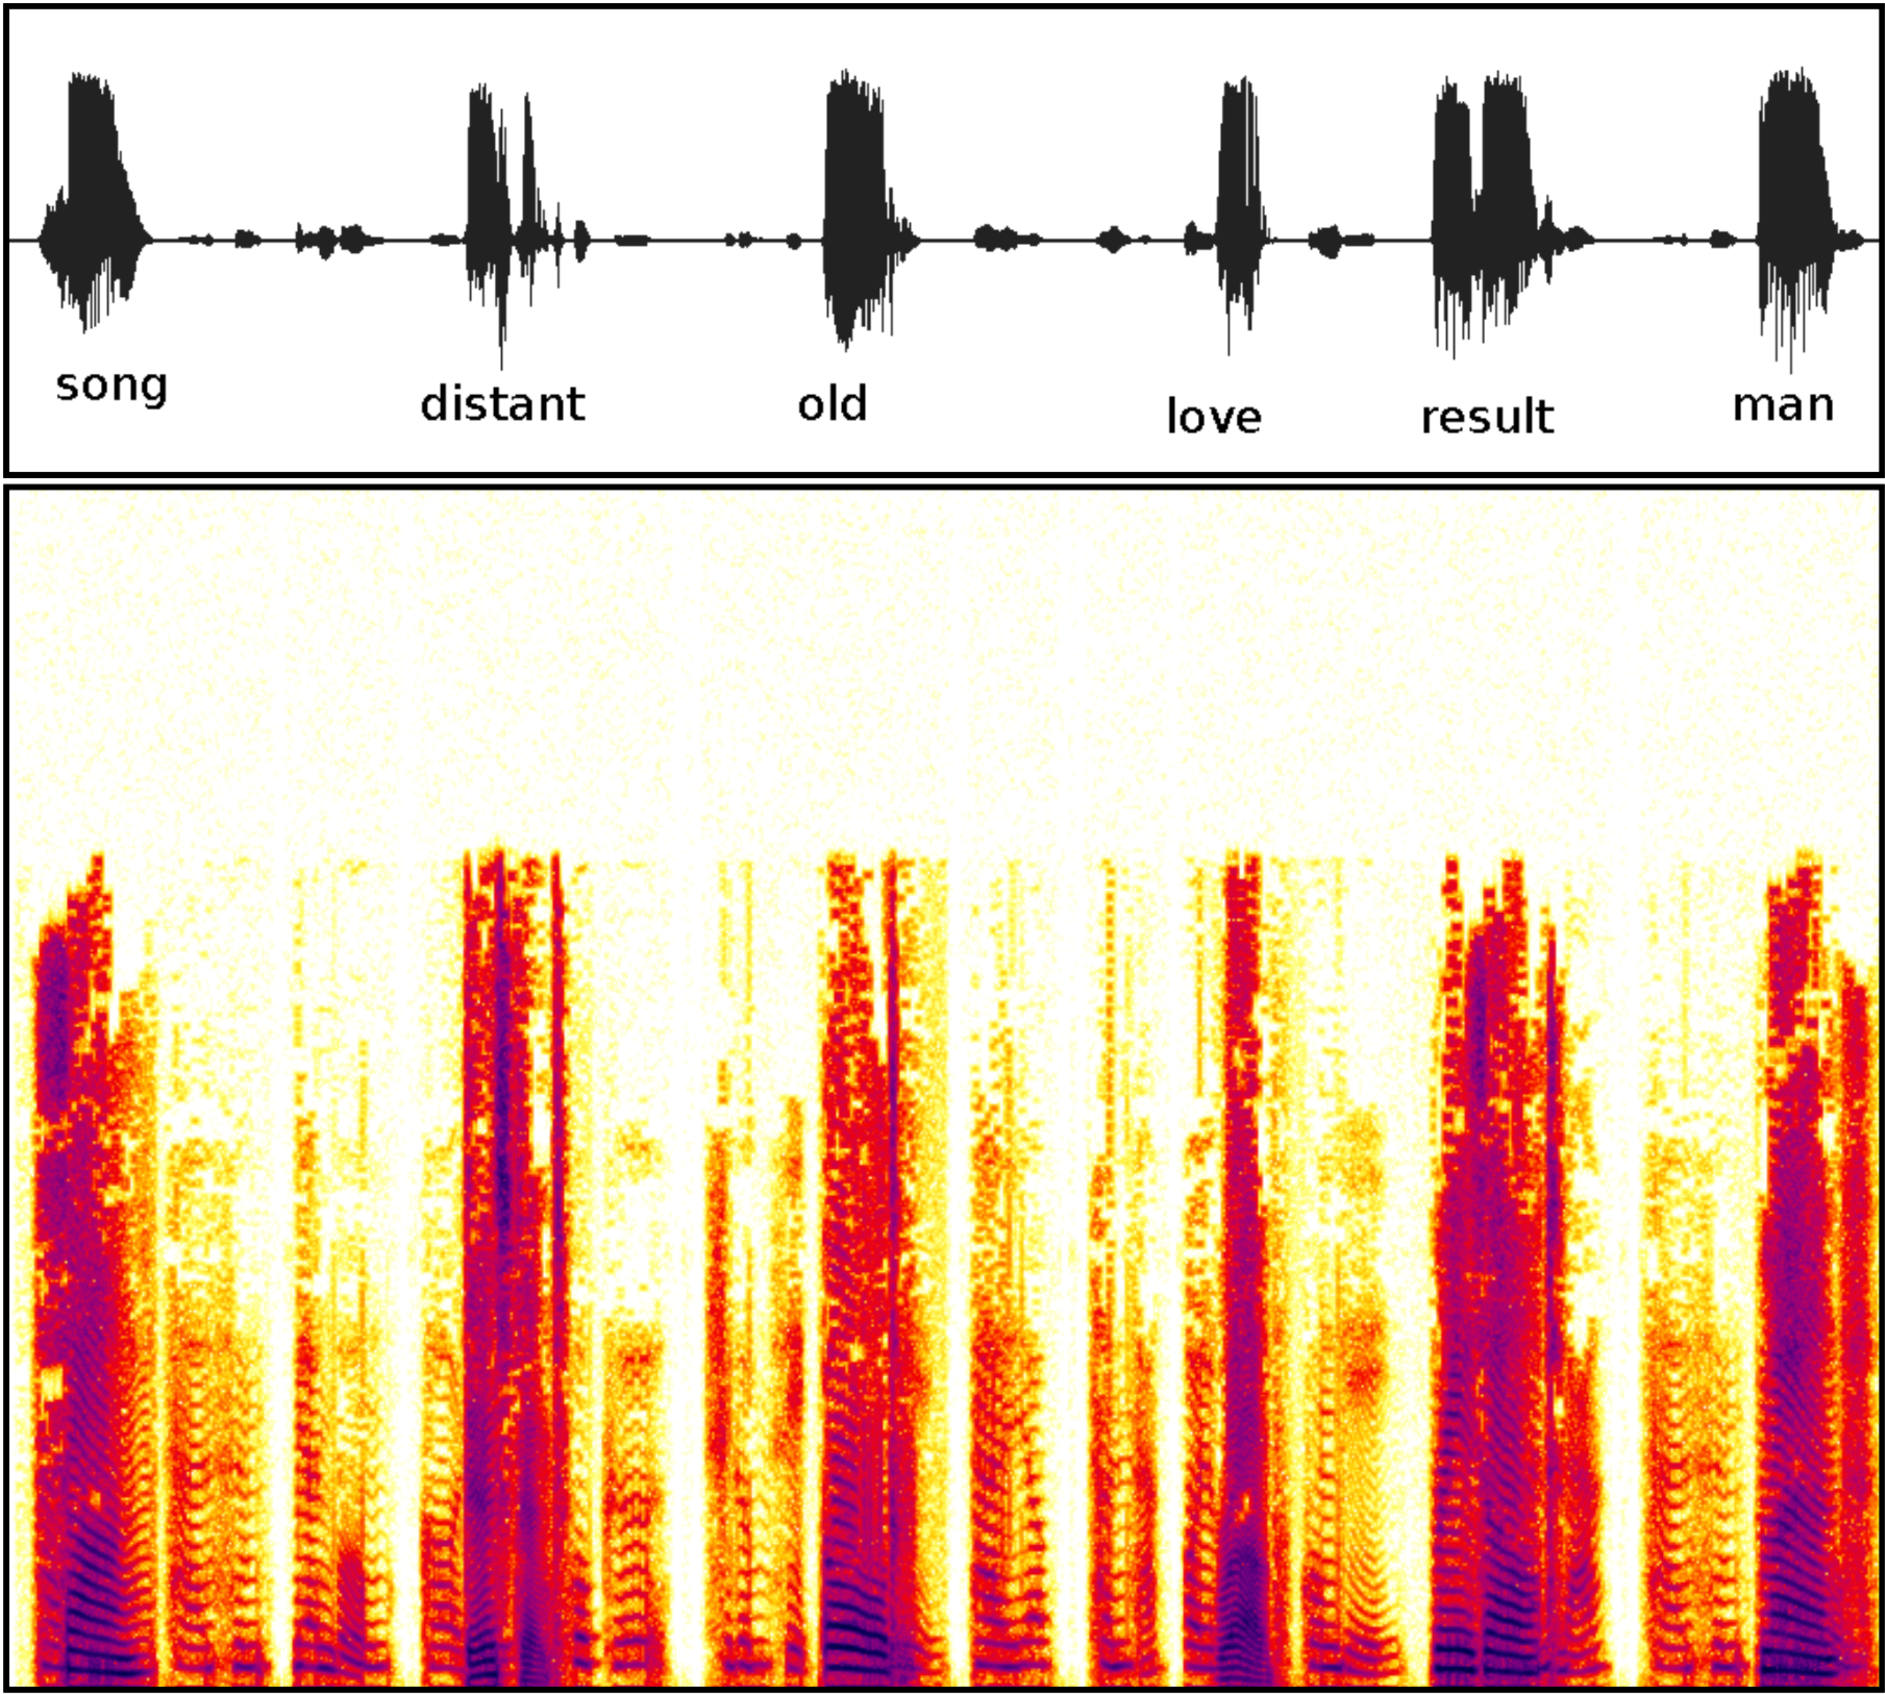
\includegraphics[width=\textwidth]{figures/live.pdf}
        \caption{Microsoft Live}
        \label{fig:live}
\end{subfigure}\hspace{0.03\textwidth} 
\begin{subfigure}{0.3\textwidth}
        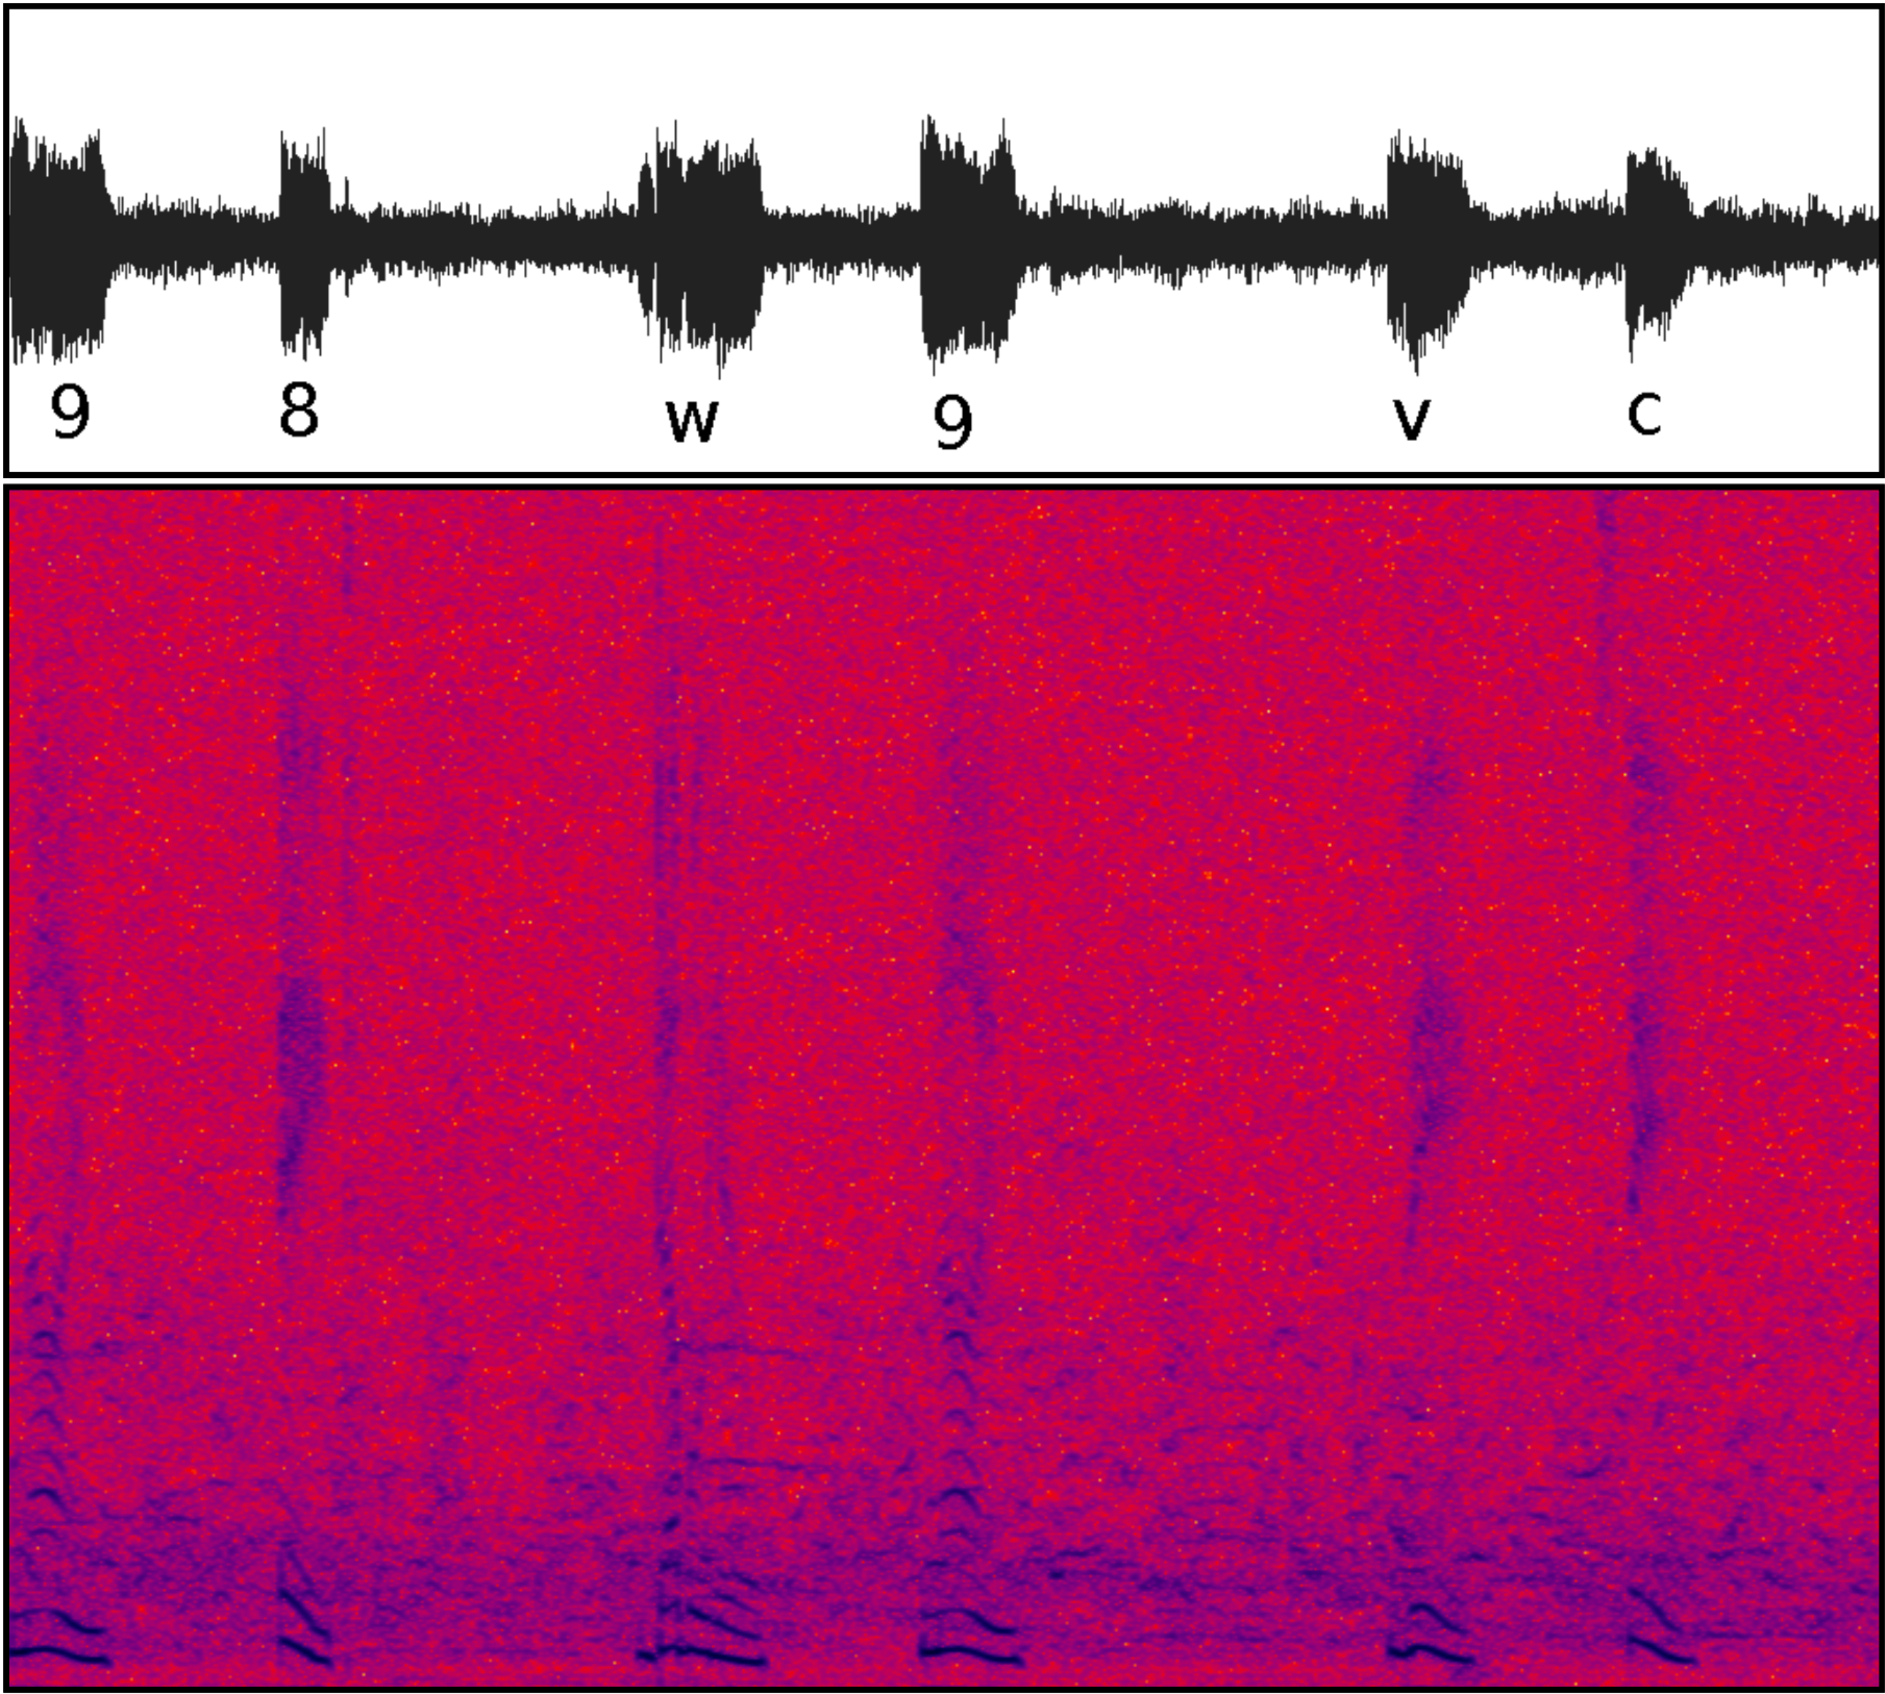
\includegraphics[width=\textwidth]{figures/secure.pdf}
        \caption{Securimage}
        \label{fig:secure}
\end{subfigure}\hspace{0.03\textwidth}
\begin{subfigure}{0.3\textwidth}
        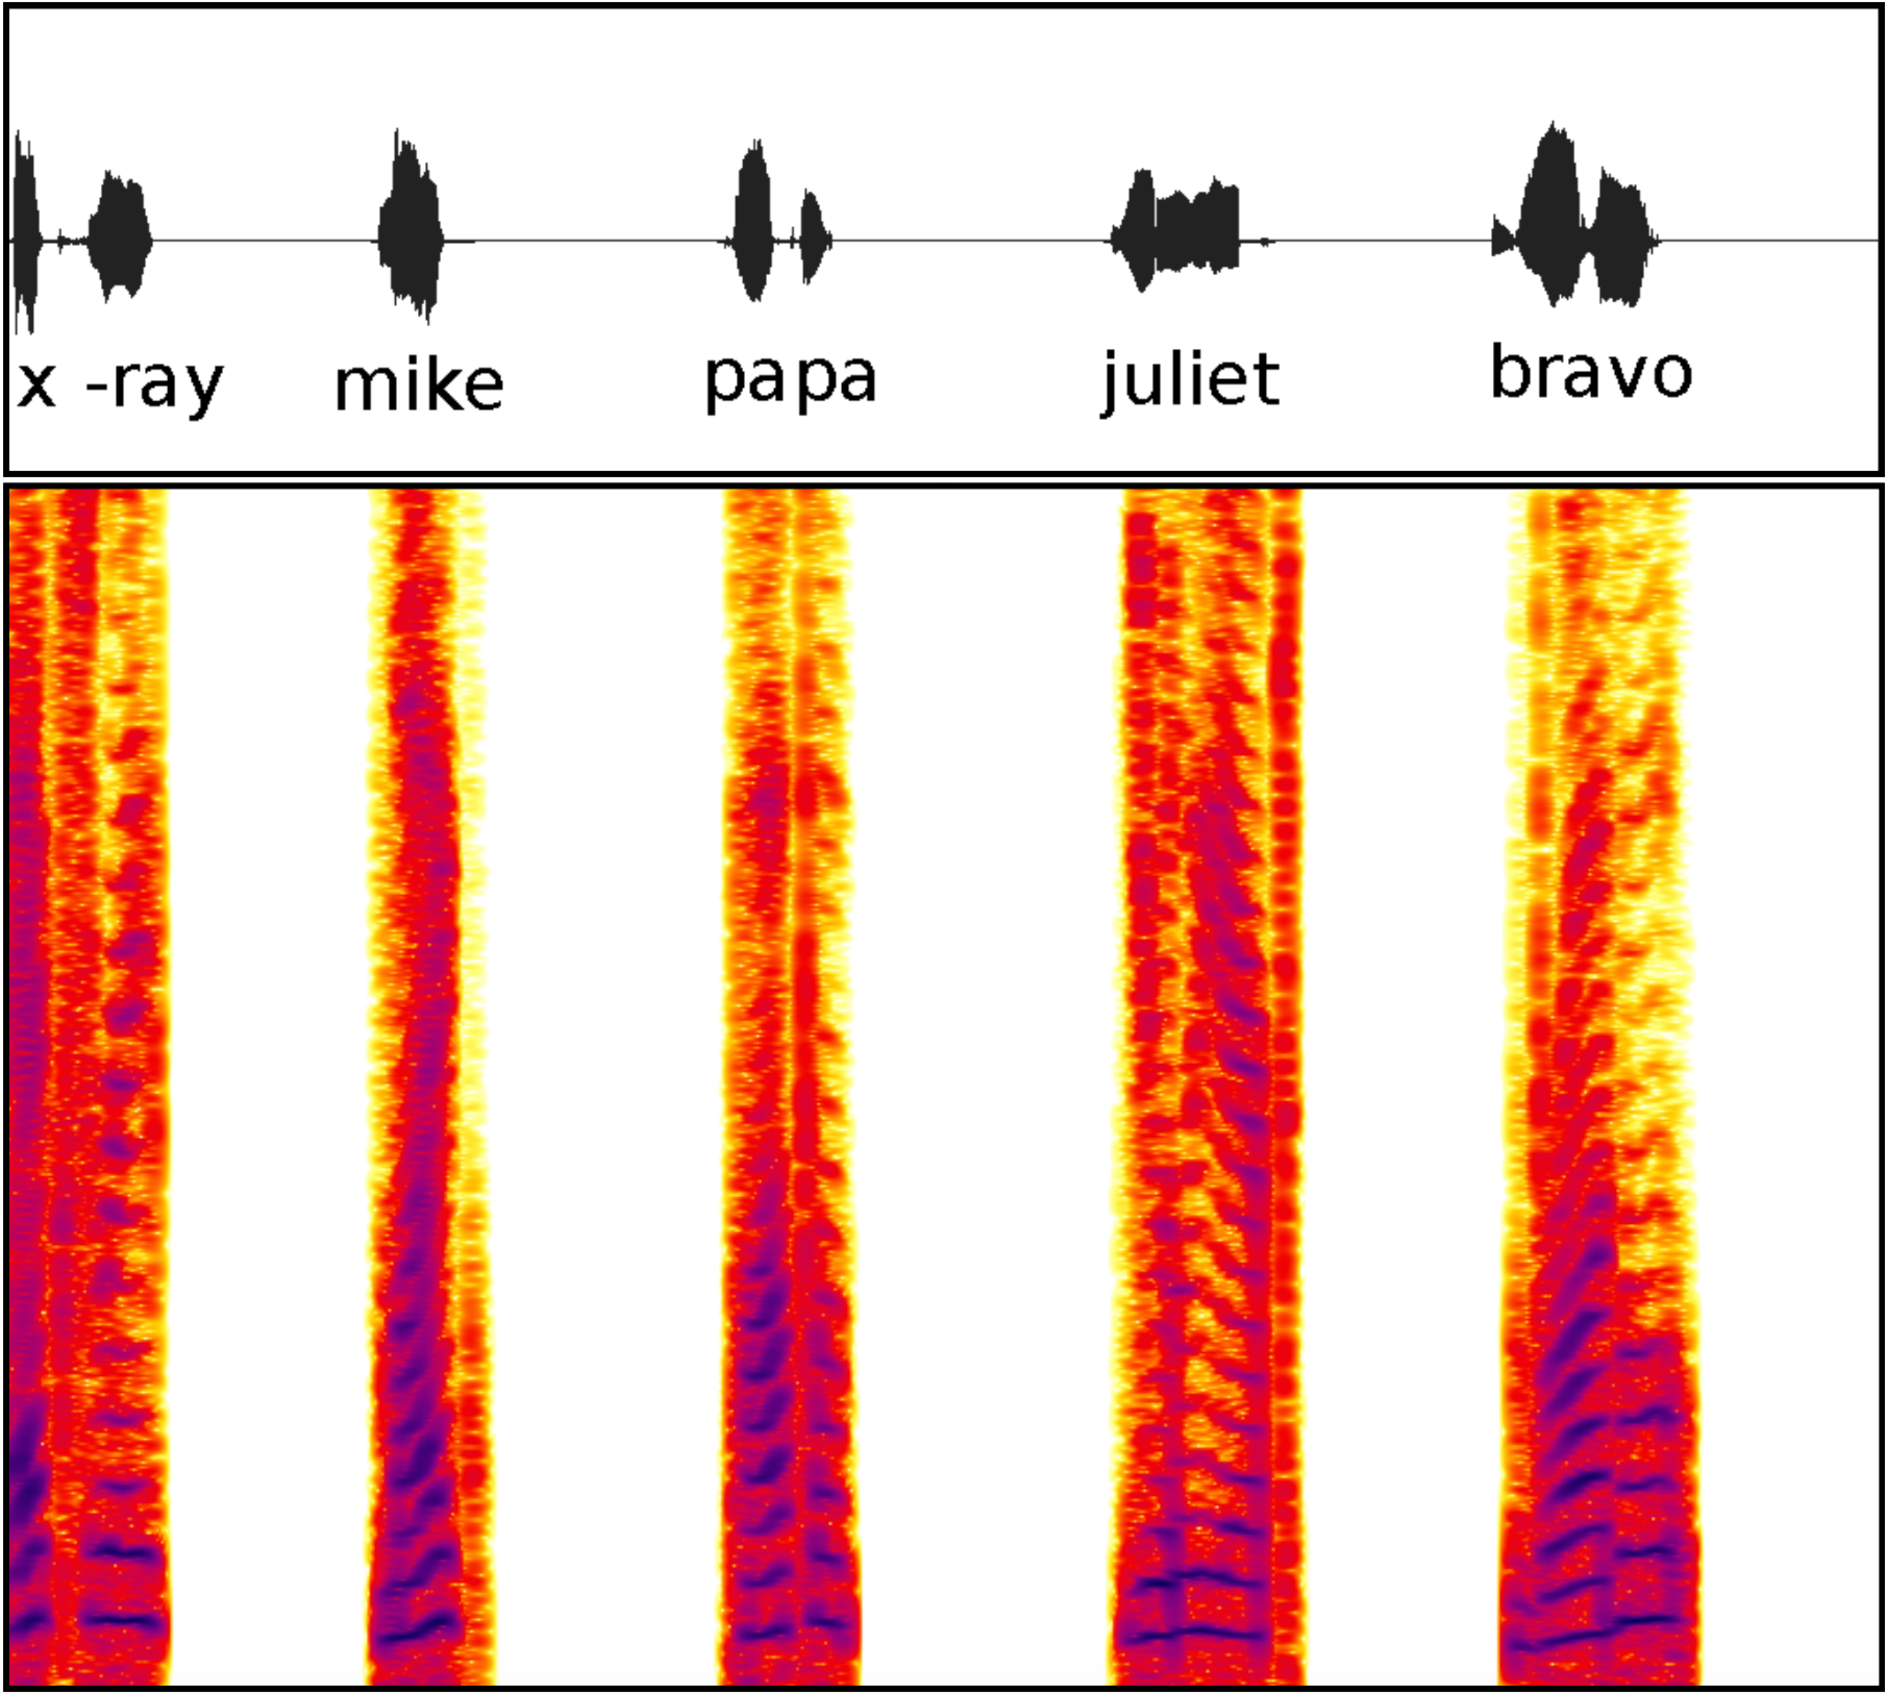
\includegraphics[width=\textwidth]{figures/telerik.pdf}
        \caption{Telerik}
        \label{fig:telerik}
\end{subfigure}
\caption{Waveforms and corresponding spectrograms for a representative sample challenge from every captcha service.}
\label{fig:examples}
\end{figure*}

\subsection{Google \re}
\label{sec:recaptcha}

Google's Recaptcha system, which is the most widely deployed captcha system,
has evolved significantly from its original form, both for adapting to publicized 
attacks (e.g.,~\cite{GoodfellowBIAS13}) and for minimizing the nuisance 
presented to users. While the audio version has not evolved as drastically from its original 
form, during our experiments there was a change in the audio challenges; we 
differentiate between the 2 versions in the remainder of the paper.

%Google provides a demo page for Recaptcha, its state-of-the-art captcha system (the version 2 of Recaptcha), 
%accessible via the following URL (https://www.google.com/\newline recaptcha/api2/demo), for anyone who wants 
%to try out the new captcha system. We used this demo page for all our tests on Recaptcha. The page connects 
%over HTTPS and does not require a login. The page initially loads a widget with a checkbox, which on clicking, 
%shows another widget with the image captcha that loads in a new iframe. The audio captcha challenge appears only 
%after clicking on the headphones-like icon in the bottom of the second widget.

\textbf{Recaptcha v2.0.} The audio challenge provided by the \re system spells out 5 digits
consecutively with little or noise, while the interval between the digits fluctuates. 
Each digit may be spoken out by the same individual (male or female), or multiple 
speakers may be employed. While the challenges do not contain background noise, certain 
spoken digits have a more distorted nature and sound drawn out or slowed down.  %Accents tend to not differ that much.

%The challenge also provides an option for the user to download the .mp3 version of the audio. The recaptcha system provides 
%a margin for error and allows up to 2 incorrect digits out of the 5. We demonstrate how this high margin for error can be 
%leveraged to get an almost 100\% accuracy value. We were able to exploit a security flaw in this system that allowed us to 
%bypass the rate limiting that was in place.
%
%The recaptcha demo page generates a new captcha challenge each time we connect to it. It behaves exactly like the recaptcha 
%v2 widget that is embedded in popular websites such as Quora, BusinessInsider, Twitter, Ticketmaster and many more, as part 
%of their account creation process. This was one of the main reasons why we chose to do our tests with the demo page, instead 
%of any particular website that employs Google's recaptcha. Our results would thus stay valid on any website that has the latest 
%recaptcha widget embedded.

\textbf{Recaptcha v2.1.} This is the latest version of \re that was released after our initial period of experiments (deployed in March 2017).
To offer a more accurate and complete picture of how the system has evolved, we include experiments against both versions.
This version is part of the latest ``Invisible \re'' version which builds upon the ``No Captcha \re'' risk analysis engine attacked in 
previous work~\cite{sivakorn:eurosp16}. This version spells out 10 consecutive digits without background noise, but also includes
recordings of digits that sound distorted.

%\textbf{Recaptcha 1.0} Although still used in many websites, Google has discontinued this version of \re since 2014.
%Furthermore, signing up for \re now will enable the newest version by default. It must be
%noted that the websites that used this version previously did not automatically upgrade to the No 
%captcha Recaptcha version, and remain open to the vulnerabilities that were fixed in the subsequent 
%version. Again, ten digits are spoken in the audio challenge and there is very little or no noise. This 
%version does not enforce any rate limiting unlike the newer versions of \re. The margin for error 
%is again 1 out of the 10 spoken digits. We have obtained \note{X} samples from the authors 
%of~\cite{meutzner2014using} so as to compare the effectiveness of our attack that uses 
%off-the-shelf speech recognition systems against previous studies that used custom
%machine learning classifiers.

\textbf{Automating.} As detailed in previous work~\cite{sivakorn:eurosp16}, \re employs various
safeguards that compliment the captcha challenges and aim to mitigate the extent of automated 
actions.

\emph{Form filling.} \re's analysis engine also detects bots by measuring the time delay between
each text box being filled in for identifying automated actions. To overcome this we introduce 
random delays between each action (the engine also flags bots that maintain a constant delay 
between actions).

\emph{Rate limiting.} One of the safeguards in place aims to throttle automated attacks by limiting 
the amount of captchas that can be solved by a single machine (similar to the token buckets approach proposed by
Elson et al.~\cite{asirra}). In Section~\ref{sec:evaluation} we describe a bug that we identified in the system
that allowed us to bypass this check.

\subsection{Apple}

Apple's captcha is encountered while signing up for a new iCloud account.
Before spelling out the audio challenge,
the voice first says ``Please enter the $n$ numbers that you hear in the textbox provided''. The 
spoken numbers consist of a total of n double digit numbers spoken by a single speaker with a synthetic/robotic voice with a pause between each double digit number.
Background noise is only present when the numbers are spoken,
and resembles a clamor of children.
The page times out after two minutes of inactivity and a pop up appears for confirmation if the user is 
still in the process of creating the account. 
%Apple does not allow downloading the audio file and is 
%loaded and played via JavaScript and not stored in any cache or temporary storage.

%To obtain the audio file for the challenge, one has to manually open the URL chrome://media-internals 
%on the Google Chrome browser. The Media Internals feature of Chrome displays three things \cite{media}:
%\begin{itemize}
%\item Everything it can dig up from the media stack about active media players. Includes buffered data, 
%    video properties, measured times between events, and a log of events.
%\item Status and volume of active audio streams. These are not yet associated with a particular tab.
%\item Cache activity, including reads from and writes to the media cache.\newline
%\end{itemize}

\textbf{Automating.} Apple has opted for certain design choices that pose obstacles to automated actions,
which we discuss below.

\emph{Obtaining audio.} By deploying their own HTML5 audio player Apple has made it 
difficult to obtain the audio recording, as opposed to other services like \re
that allow a straightforward fetching of the mp3 file. As a workaround, we access 
the browser's media stack\footnote{Through chrome://media-internals.} and obtain the 
audio recording in base64 format, this is converted to a wav format file and uploaded to the voice recognition services for solving. 

\emph{Form filling.} Form elements are not accessible via HTML IDs/tags; instead we enumerate them 
using XPath (input[@type='text']), and access them according to attribute values. The username needs to be 
unique every time as the username validation script runs once the username has been input into the textbox.
Furthermore, the system requires mouse interaction for actually accessing an element, otherwise the 
form's validation script will not execute if the password boxes have not been ``touched'',  i.e, accessed via mouse. We automate this
process using PyWinAuto~\cite{pywinauto}. As no other form elements require this form of explicit interaction,
we hypothesize that there is an additional script that runs a check whether the password is legitimate or conforms 
to the pattern expected by the service and this is why that additional interaction is required.

Apart from the two aforementioned complexities, Apple does not employ any form of rate limiting in 
the form of checking for standardized behavior, or considering an IP address as suspicious if its behind a proxy, or VPN.
Furthermore, unlike Google \re it does not present harder challenges or ban the IP address after several attempts. 

\textbf{Pre-processing.} We remove the spoken instructions at the beginning of the audio file
before it is sent to the service.

\begin{table*}[t]
\centering
\caption{Attack accuracy for each speech recognition service and accent configuration, against the audio captcha services we evaluated.}
\begin{tabular}{lccccc}
\toprule
&\multicolumn{5}{c}{\textbf{Speech Recognition Service (Accent)}}\\
\cmidrule{2-6}
\textbf{Captcha Service}& \textbf{Wit}& \textbf{IBM (US)} & \textbf{ IBM (UK)} & \textbf{Google (US)} & \textbf{Google (UK)} \\
\hline
Recaptcha v2.0 & 67.1\% (671/1000) & 95.8\% (958/1000) & 67.2\% (672/1000) & \textbf{98.3\%} (983/1000) & 81.6\% (816/1000) \\
\rowcolor{Gray}
Recaptcha v2.1 & -  & - & -  & \textbf{83.9\%} (1786/2128) & - \\
Apple  & 0\% (0/365)  & 2.3\% (6/260) & 6.8\% (17/251) & 35.8\% (126/352) & \textbf{52.8\%} (143/271) \\
\rowcolor{Gray}
BotDetect  & 1.23\% (11/894)  & 1.38\% (19/138) & 6.67\% (12/180) & \textbf{9.5\%} (102/1067)  & 6.65\% (79/1187) \\
Captchas.net  & 0\% (0/1008) & 1.1\% (9/778)  & 0.3\% (3/1010)  & 2.7\% (16/593) & \textbf{22.3\%} (230/1030) \\
\rowcolor{Gray}
Microsoft Live & \textbf{24.7\%} (71/287) & 10.6\% (23/216)  & 13.1\% (28/213)  & 21.2\% (28/132)  & 18.6\% (27/145) \\
Securimage  & 0\% (0/1000)  & 0\% (0/1000) & 0\% (0/1000) & 0.1\% (0/1000) & \textbf{3\%} (30/1000) \\
\rowcolor{Gray}
Telerik  & 21.2\% (142/668)  & \textbf{97\%} (452/466) & 12.9\% (47/364) & 74.2\% (150/202) & 49.3\% (112/217) \\
\bottomrule
\end{tabular}
\label{tab:combinations}
\end{table*}


\subsection{BotDetect}
%BotDetect offers free and paid versions of its captcha system. In the free version, the 
%service has several limitations, like the audio challenge is not fully functional most of 
%the times. There is a 50\% chance that the audio challenge is replaced with an audio file 
%that speaks "Sound Demo". BotDetect offers libraries for integration with .NET, Java, ASP 
%and PHP based websites. The demo page of BotDetect can be accessed here: 
%\url{https://captcha.com/demos/features/captcha-demo.aspx}.

The audio challenge contains the spoken version of the digits and letters shown in the text captcha.
This captcha service offers many customization options during its integration in a website. For instance, 
the number of alphanumeric characters in the challenge can be chosen between
1-13 (the default being a random selection between 4-6). The background noise can be random or selected from one of 
the 10 noise types and the sound type can be customized as well (choice of 8 Bit Mono audio or 16 Bit 
Mono audio). The default demo version that we experimented with contains intermittent electronic noise that 
coincides with the spoken letters. The background noise can be characterized as microphone noise. 

Their demo site, unlike the \re demo page, does not use any form of rate limiting or
time out check. The demo page also does not react differently after repeated accesses and hence does not a VPN 
or proxy to hide behind. Obtaining the audio sample is trivial as there is a URL available
on the source of this page pointing to the network object. We do 
not add delays for accessing the form elements as it is not checked on the demo page. As the demo page does not provide other
checks apart from the captcha itself, someone utilizing this service would need to implement
additional safeguards.

\textbf{Pre-processing.} The audio file obtained is in \texttt{wav} format and needs to be converted to \texttt{flac} only for 
the Google Speech solver. We do not apply any other form of processing apart from that.


\textbf{Post-processing.} Based upon the audio transcript received and the audio solvers chosen, common erroneous transcriptions
that we observed were replaced with their homophones.  As we know the alphanumeric pattern
expected, we are able to accurately ascertain what errors each service is likely to make.

%We found that this service is used widely, and we encountered it on the Visa status check 
%page of US CEAC website here: https://ceac.state.gov/ceacstattracker/status.aspx \newline

\subsection{Captchas.net}

Captchas.net started in 2004 offers implementation and easy integration for PHP, ASP, Perl, 
Python, JSP and Ruby. It is a free service, but shows a watermark on the images of the text challenges 
which can be removed by subscribing to the paid version. 
The audio challenges employ the NATO phonetic alphabet, and the user has to enter the corresponding letters.
For instance, ``RIPAZH'' would be read out as 'Romeo India Papa Alpha Zulu Hotel' and the user is expected 
to enter the first letter of each uttered word. The audio challenges contain little background noise during the 
spoken words. However, the words themselves are distorted and sound like digitally synthesized speech.

The demo page does not provide any form of rate limiting or detection of suspicious activity at the client side, 
and the demo page does not flag repeated accesses from the same IP address as suspicious, therefore there was no need 
to employ a proxy or VPN during our experiments. Obtaining the audio file is again trivial as a URL is contained in the 
HTML source for the network object, which can be easily retrieved. Furthermore, it does not look for timing delays between 
accessing form elements. As with BotDetect, it does not check for automated behaviour apart from employing the captcha, 
and anyone utilizing this service would need to develop their own safeguards.

\textbf{Pre-processing.} The audio file obtained is an \texttt{mp3} and is once again converted to \text{flac} for the Google Speech solver, 
and is required to be converted to wav for the other two solvers. The file requires no additional pre-processing. However, we do
set the Google Solver to look for certain words ie send the phonetic NATO alphabet phrases with the request for transcription. 
This allows for the google solver to more accurately pick transcriptions and with higher confidence.  The audio file has additional 
near 5 seconds of empty space at the end of each audio file which we chop off before sending as well.


\textbf{Post-processing.} As before, the cloud speech services transcribe certain of the NATO phrases erroneously and we find have identified 
suitable homonyms for each and replace them. We take the first letter of each of the words transcribed as the captcha solution.

%For both the text and the audio challenges, 
%Captchas.net follows the following method to validate the response:
%
%\begin{itemize}
%\item Both the client server and Captchas.net's server share a common secret key.
%\item The secret key and a random string sent by the client are used to generate the password.
%\item The password is computed by Captchas.net's server to generate the image and by the client server to validate the user's input.
%\end{itemize}


\subsection{Live.com}

Microsoft's Live domain provides access to other Microsoft services, including
OneDrive, Bing, MSN, Office, Skype, Outlook.com, Xbox Live, etc. The captcha is 
encountered while registering for a new account. The audio challenge contains random English 
words. On average they are 5-letter words and 5-7 such words are spoken per challenge, which must be typed by the user.
The words are spoken by 2 different people - one female and one male. The background noise 
is from speakers talking in a foreign language.

As this is not a demo page but an actual account creation page, it employs rate limiting and other safeguards; however, it 
does not consider repeated accesses from the same IP address as suspicious. Hence, there is no need to use a proxy. 
We create a new random username for every single experiment, and simulate mouse interaction with the password box to 
trigger the password validation scripts. %Accessing script elements on the page is harder as they have utilized class names 
%with spaces in them leading it to be harder to reference them via simple xpath. 

\textbf{Pre-processing.} The audio file obtained is through accessing the media-stack as described in the Apple section, 
and the file obtained is encoded in Base64, which we convert to the desired format for each of the cloud speech recognition services.

\textbf{Post-processing.} We do minimal post-processing, as the service uses dictionary words, and there is no reliable regular 
pattern of mistaken transcriptions that we can leverage for increasing the attack's accuracy.

%although we found that the number of words spoken out by the female voice are much higher. In our opinion, it provided better accessibility 
%to visually impaired users as they can press '1' on their keyboard to play or repeat the audio challenge 
%and by requesting a new challenge using the button labeled 'New' on the interface, the focus is set to the 
%response box automatically.

\subsection{Securimage}

Securimage is an open source captcha system that has been under active development and maintenance 
since 2005. It offers plugins/modules for major content management systems, with a lot of customization 
options for both image and audio based challenges. For each audio challenge, the system generates a WAV 
file from a corpus of audio files of 26 alphabets (A-Z) and 10 digits (0-9). The digits and alphabets are 
spoken by a single person. The audio is generated by picking 6 word/digit files at random, combining them and adding one 
of the 5 noise files. The default number of digits/characters per challenge is 6, but this can 
be customized while implementing the library. The entire audio recording contains background noise resembling
human clamor.
%Some other customization options are that one can 
%specify a word list for the challenges and using a read-aloud math puzzle that is to be solved 
%by the user.

Secureimage has a demo page, and does not employ any form of rate limiting and detection on its own nor does it 
consider repeated accesses from the same IP address as suspicious. Similar to captchas.net and BotDetect we not add
additional delays for accessing each of the form elements. The audio file is easily accessible via the URL contained in the page.

\textbf{Pre-processing.} The audio file obtained is in \texttt{wav} format, which we convert to the desired format. 
The audio file is otherwise not edited.

\textbf{Post-processing.} This service uses only letters of the alphabet, hence we are able to identify regular mistakes in the 
transcriptions obtained from each service, and map them to their correct letter transcriptions.


\subsection{RadCaptcha by Telerik}

RadCaptcha is a captcha service by Telerik that is built especially for ASP.NET 
web applications. 
%RadCaptcha and 90+ other controls are part of UI for ASP.NET AJAX, 
%a comprehensive toolset that take care of the common functionality of a ASP based
%CMS like Sitefinity \cite{radcaptcha}. 
%It is also a part of a feedback form for the 
%HR website of UIC, where we discovered this captcha. It can be seen here: https://www
%.hr.uic.edu/cms/One.aspx?pageId=356957\newline
RadCaptcha's audio challenge contains digits (0-9) and the NATO phonetic alphabet. It is 
spelled out by a single speaker and there is almost no background noise in the audio. 
%The 
%audio is not available to download explicitly, but is present on the DOM of the web page 
%in an <audio> tag, from which the URL of the audio file can be easily grabbed. 
One of the customizations provided by the service is a throttling measure, which requires the form to 
be displayed to the user for a particular number of seconds before an answer will be considered as 
human-submitted. However, this setting is left up to the developer who incorporates the captcha 
service on the target web page.

Telerik also has a demo page, and does not employ any form of rate limiting nor does it consider repeated 
accesses from the same IP address as suspicious. ALso, there is no need for additional delays when accessing 
each of the form elements. The audio file is easily accessible via its URL.

\textbf{Pre-processing.} The audio file obtained is in \texttt{wav} format, which we convert to the desired format.
The audio file is otherwise not edited.

\textbf{Post-processing.} This service uses only the NATO alphabet, and we find relevant homonyms for the common mistakes.
We take the first letter of each of the words transcribed as the captcha solution.


%\begin{table*}[t]
%\centering
%\caption{Accuracy of different speech recognition services and accents against the audio captcha services we evaluated.}
%\begin{tabular}{lccccc}
%\toprule
%&\multicolumn{5}{c}{\textbf{Speech Recognition Service (Accent)}}\\
%\cmidrule{2-6}
%\textbf{Captcha Service}& \textbf{Wit}& \textbf{IBM (US)} & \textbf{ IBM (UK)} & \textbf{Google (US)} & \textbf{Google (UK)} \\
%\hline
%Recaptcha v2.0 & 67.1\% (671/1000) & 95.8\% (958/1000) & 67.2\% (672/1000) & \textbf{98.3\%} (983/1000) & 81.6\% (816/1000) \\
%\rowcolor{Gray}
%Recaptcha v2.1 & -  & - & -  & \textbf{83.9\%} (1786/2128) & - \\
%Apple  & 0\% (0/365)  & 2.3\% (6/260) & 6.8\% (17/251) & 35.8\% (126/352) & \textbf{52.8\%} (143/271) \\
%\rowcolor{Gray}
%BotDetect  & 1.23\% (11/894)  & 1.38\% (19/138) & 6.67\% (12/180) & \textbf{9.5\%} (102/1067)  & 6.65\% (79/1187) \\
%Captchas.net  & 0\% (0/1008) & 1.1\% (9/778)  & 0.3\% (3/1010)  & 2.7\% (16/593) & \textbf{22.3\%} (230/1030) \\
%\rowcolor{Gray}
%Microsoft Live & 24.7\% (71/287) &  &  & 21.2\$ (28/132)  & 18.6\$ (27/145) \\
%Securimage  & 0\% (0/1000)  & 0\% (0/1000) & 0\% (0/1000) & 0.1\% (0/1000) & \textbf{3\%} (30/1000) \\
%\rowcolor{Gray}
%Telerik  & 21.2\% (142/668)  & \textbf{97\%} (452/466) & 12.9\% (47/364) & 74.2\% (150/202) & 49.3\% (112/217) \\
%\bottomrule
%\end{tabular}
%\label{tab:combinations}
%\end{table*}
%
\section{Experimental Evaluation}
\label{sec:evaluation}

In this section we present the results from our extensive experiments again 
the audio captcha services presented in Section~\ref{sec:services}.

\textbf{Attack accuracy.} Table~\ref{tab:combinations} presents the accuracy obtained by each speech recognition service 
against the audio captcha services. In cases where the speech recognition service has the option to select an accent,
we experiment with both American and British English. For \re v2.1 that was released during our experiments, we run
an extensive experiment using only the configuration that had the best results again v2.0, so as to minimize the 
overhead of our experiments on the \re service.

Surprisingly we find that for every single captcha scheme, at least
one of the speech recognition services is able to solve more challenges than the 1\% threshold, thus, \emph{practically 
rendering all captcha schemes broken.} Nonetheless, there is significant variance, not only across captcha schemes, but
the accuracy obtained by each speech recognition engine for a specific captcha service.
The most alarming finding is that \system achieves one of the best results \re, the most widely deployed captcha service.
When considering the 70.78\% attack accuracy reported for the image challenges of v2.0~\cite{sivakorn:eurosp16},
it becomes apparent that audio challenges weaken the overall security offered by \re, as fraudsters can target 
audio captchas for deploying highly successful attacks. 
The Apple and Microsoft Live captchas that protect their account creation process, are also highly susceptible to 
automated attacks, as our approach correctly solves up to 52.8\% and \note{X\%} respectively.

As expected, the services that have more noise, prove to be more robust.
However, despite the presence of noise impacting the accuracy of the transcription process for all the respective captcha schemes
none of the services is completely impervious to our attacks. Nonetheless, we
found that the audio captchas from Securimage are the most robust due to the presence of background semantic noise,
as \system was only able to solve 3\% of the challenges when using Google's Speech API and the British English accent
configuration. Another interesting observation was that no single speech recognition system or configuration
was consistently more accurate across all captchas; however, Google's speech recognition achieved the best
results for \note{X} of the captcha schemes. While attackers could increase the attacks' accuracy
by first pre-processing the audio challenges so as to reduce the noise, the motivation behind our study is to 
demonstrate how attackers can employ off-the-shelf systems for breaking existing captcha systems.
Based on these results, we find that \system would be an effective replacement to the human solvers employed by
captcha solving services, as humans are often troubled by audio challenges~\cite{captchas-are-hard}.


\begin{table}[t]
\centering
\caption{Average solution time (seconds) for each recognition service and accent against the audio captcha services we evaluated.}
\begin{tabular}{lccccc}
\toprule
&\multicolumn{5}{c}{\textbf{Speech Recognition Service}}\\
\cmidrule{2-6}
& & \textbf{(US)} & \textbf{(UK)} & \textbf{(US)} & \textbf{(UK)} \\
\textbf{Captcha}&  \textbf{Wit} & \textbf{IBM} & \textbf{IBM} & \textbf{Google} & \textbf{Google} \\
\hline
Recaptcha v2.0 & 13.85s & 10.56s  & 12.25s & \textbf{18.46s} & 20.41s \\
\rowcolor{Gray}
Recaptcha v2.1 & -  & -  & - & \textbf{43.24s} & - \\
Apple  & 36.4s & 33.4s  & 34.7s & 15.5s & \textbf{13.9s} \\
\rowcolor{Gray}
BotDetect  & 5.53s  & 4.21s & 5.72s & \textbf{3.40s} & 3.05s \\
Captchas.net  & 19.92s  & 14.62s  & 15.65s  & 7.56s & \textbf{7.79s} \\
\rowcolor{Gray}
Microsoft Live & 14.37s  &  &  & 10.52s  & 9.07s \\
Securimage  & 34.31s & 23.60s & 25.10s  & 27.29s & \textbf{35.28s} \\
\rowcolor{Gray}
Telerik  & 7.53s & \textbf{5.56s} & 6.65s & 3.86s & 3.83s \\
\bottomrule
\end{tabular}
\label{tab:solution_time}
\end{table}

\textbf{Solution time.} In Table~\ref{tab:solution_time} we include the average time required by each speech recognition 
service for returning a transcription of the audio captcha. The bold values denote the combination that achieved the highest 
accuracy for that captcha scheme. As can be seen, there is considerable variation on the time required by the different speech 
recognition services for each captcha scheme. \system solves the Telerik challenges in the least amount of time, while both
Apple and Securimage require considerably more effort to obtain the transcription. While Google Speech requires $\sim$18.4 
seconds on average for most accurate attacks against \re v2.0, that increases significantly for v2.1 as it has the longest
audio challenges (see Table~\ref{tab:money} below). Interestingly, in several cases the speech recognition systems return
a transcription in less time than the actual duration of the challenge, resulting in very efficient automated attacks.

%\note{How many mistakes allowed for a correct answer?}

\textbf{Rate limits and economic analysis.} Our study's goal is to explore the feasibility of low-cost attacks 
against popular captcha services; thus, the scale of such an attack is naturally constrained by the rate
limiting enforced by the speech recognition APIs. While an attacker could build an offline solver
using a deep learning framework like TensorFlow~\cite{abadi2016tensorflow}\footnote{Researchers have already
released prototypes that build on Tenserflow: {https://github.com/mozilla/DeepSpeech}.} to overcome this constraint,
our threat model explicitly includes non-sophisticated attackers that do not develop or train their own 
classifiers. As such, the rate limits of each speech recognition service become relevant as they could
constrain our attacks.

\begin{table}[t]
\centering
\caption{Attacker's estimated daily profit for each captcha service, when using one Google Speech API account
(with the most accurate accent configuration for that captcha scheme).}
\begin{tabular}{lccc}
\toprule
& \textbf{Captcha} & \textbf{Expected} & \textbf{Daily} \\
\textbf{Captcha}&  \textbf{Duration} & \textbf{Solutions} & \textbf{Profit} \\
\hline
Recaptcha v2.0 & 7 sec & 242,413 & \$485.3 \\
\rowcolor{Gray}
Recaptcha v2.1 & 15 sec & 96,652 & \$193.3 \\
Apple  & 14 sec & 65,170 & \$130.3 \\
\rowcolor{Gray}
BotDetect  & 6 sec & 28,215 & \$54.7 \\
Captchas.net & 14 sec & 27,524 & \$55 \\
\rowcolor{Gray}
Microsoft Live & 11 sec &  & \\
Securimage & 10 sec & 5,184 & \$10.3 \\
\rowcolor{Gray}
Telerik & 7 sec & 188,892 & \$366.3 \\
\bottomrule
\end{tabular}
\label{tab:money}
\end{table}

Surprisingly, these services have very lax limits that would enable fraudsters to misuse
them for maintaining large scale audio captcha solving campaigns. For instance, Google's Speech API allows up
to 250,000 requests per day, where multiple audio files can be submitted per request, allowing for a maximum of
480 hours of audio processing.\footnote{https://cloud.google.com/speech/limits}
In Table~\ref{tab:money} we provide a rough estimation of the profit that an attacker could yield against 
each captcha service per day using a single Google API account. We assume a lower end market price of \$2 
per 1,000 solved captchas, and calculate the number of solved captchas based on the length of audio challenges 
and the highest accuracy achieved by a Google Speech solver (see Table~\ref{tab:combinations}) for each service.
There is a large variance between the potential profit for each captcha service due to the difference in challenge
durations as well as the attacks' accuracy. Deploying a solving service for \re would be a highly lucrative
operation given its prevalence.
It is important to note, however, that these calculations assume that the attacker 
is not constrained by other forms of rate limiting (e.g., IP-based limits). Given the workarounds employed
by existing captcha solving services (e.g., proxies, botnets, etc), in practice these limitations will not 
pose an insurmountable obstacle.

On the other hand, IBM Watson allows 1 free month per account.\footnote{https://www.ibm.com/watson/services/natural-language-classifier/}
Finally, Wit does not have an explicit rate limit. However, it is open to commercial
apps and requires notification for rates approaching one request per second. As all three services
only require an email address for creating an account, attackers could trivially register 
new email addresses periodically for increasing their overall allowed throughput.

%In comparison Clarifai,
%the most accurate image annotation service used against \re~\cite{sivakorn:eurosp16}, only allows 5,000
%free operations per month\footnote{https://developer.clarifai.com/pricing/}.


%\textbf{Solution flexibility.} \note{How many wrong digits allowed per service?}

\begin{figure*}[t]
\begin{subfigure}{0.75\textwidth}
    \centering
    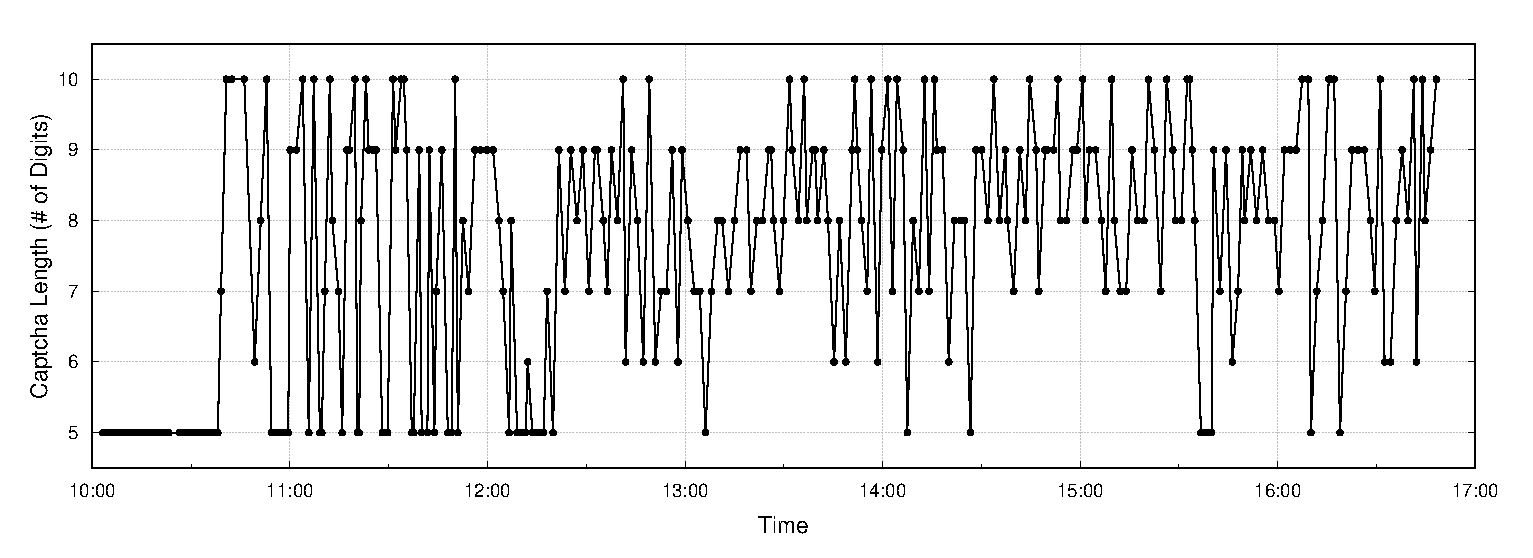
\includegraphics[width=1\textwidth]{figures/captcha_length.eps}
    \label{fig:length_time}
\end{subfigure} %\hspace{0.03\textwidth}
\begin{subfigure}{0.2\textwidth}
    \centering
    %\caption{Average solution time for each recognition service and accent against the audio captcha services we evaluated.}
    \label{tab:length}
    \begin{tabular}{lc}
    \toprule
    \textbf{Digits} & \textbf{\# of Captchas} \\
    \hline
    5 & 95 (31.3\%) \\
    \rowcolor{Gray} 
    6 & 14 (4.6\%) \\
    7 & 34 (11.2\%) \\
    \rowcolor{Gray} 
    8 & 51 (16.8\%) \\
    9 & 68 (22.4\%) \\
    \rowcolor{Gray} 
    10 & 41 (13.5\%)\\
    \bottomrule
    \end{tabular}
\end{subfigure}
\caption{Variation of audio captcha length in \re v2.0 over time.}
\label{fig:length}
\end{figure*}

\textbf{\re.} While our study aims to evaluate the robustness of many popular audio captcha schemes,
Google's \re is the most prevalent captcha service, so we further elaborate on those experiments 
and offer more interesting details and findings.

\emph{Bypassing rate limits.} As aforementioned in Section~\ref{sec:recaptcha}, \re enforces 
rate limiting to prevent large scale attacks from a small number of machines. While in practice
captcha solving services employ proxies~\cite{captcha_proxies} and botnets (e.g., KoobFace~\cite{captcha_solvers}) 
to overcome such limits, we further explored this mechanism during our experiments. Initially,
we employed a straightforward approach of circulating through a list of valid User Agent strings,
so as to masquerade as numerous computers connecting from a single IP address (e.g., users behind a NAT).
However, in that case \re would enforce the same limit. Surprisingly, though, we found that if we 
supplied a bogus nonsensical User Agent we were able to completely bypass the rate limiting,
and only faced issues when issuing many concurrent solvers (which could appear as a potential DDoS attempt).
%solving  well over a thousand captchas per day from a single IP address. 
We surmise that a bug in the risk analysis
system does not enforce the check on the other aspects of the request (e.g., IP address, HTTP cookies) when
it encounters an ``invalid'' User Agent.\footnote{This issue has now been fixed.}
%This incident 
%further highlights how seemingly complex captcha services ]

\emph{Adaptive length}.
While by default the length of \re v2.0 was 5 digits, we found %that after multiple captcha_lengthptcha solutions by our system,
that \re would adapt when facing a large amount of requests from our system (when not ).
Specifically, the system adapts by returning captchas with more digit so as to impact automated attacks.
In Figure~\ref{fig:length} we present a representative experiment that depicts the number of digits in the captchas
processed by our system over the course of 7 hours. The first 49 captchas all contained 5 digits, whereas the length
changed in a seemingly random fashion. As can be seen by the breakdown statistics in the figure, apart from the default
version with 5 digits, the most common variation we came across contained 9 digits. 
%Overall, out of the 303 challenged processed in the experiment, 95 (31.3\%)
%had a length of 5, 14 (4.6\%) had 6 digits, 34 (11.2\%) had 7, 51 (16.8\%) had 8 digits, 68 (22.4\%) had 9, and 41 
%(13.5\%) had 10 digits.

\begin{figure*}[tp]
\begin{subfigure}{0.24\textwidth}
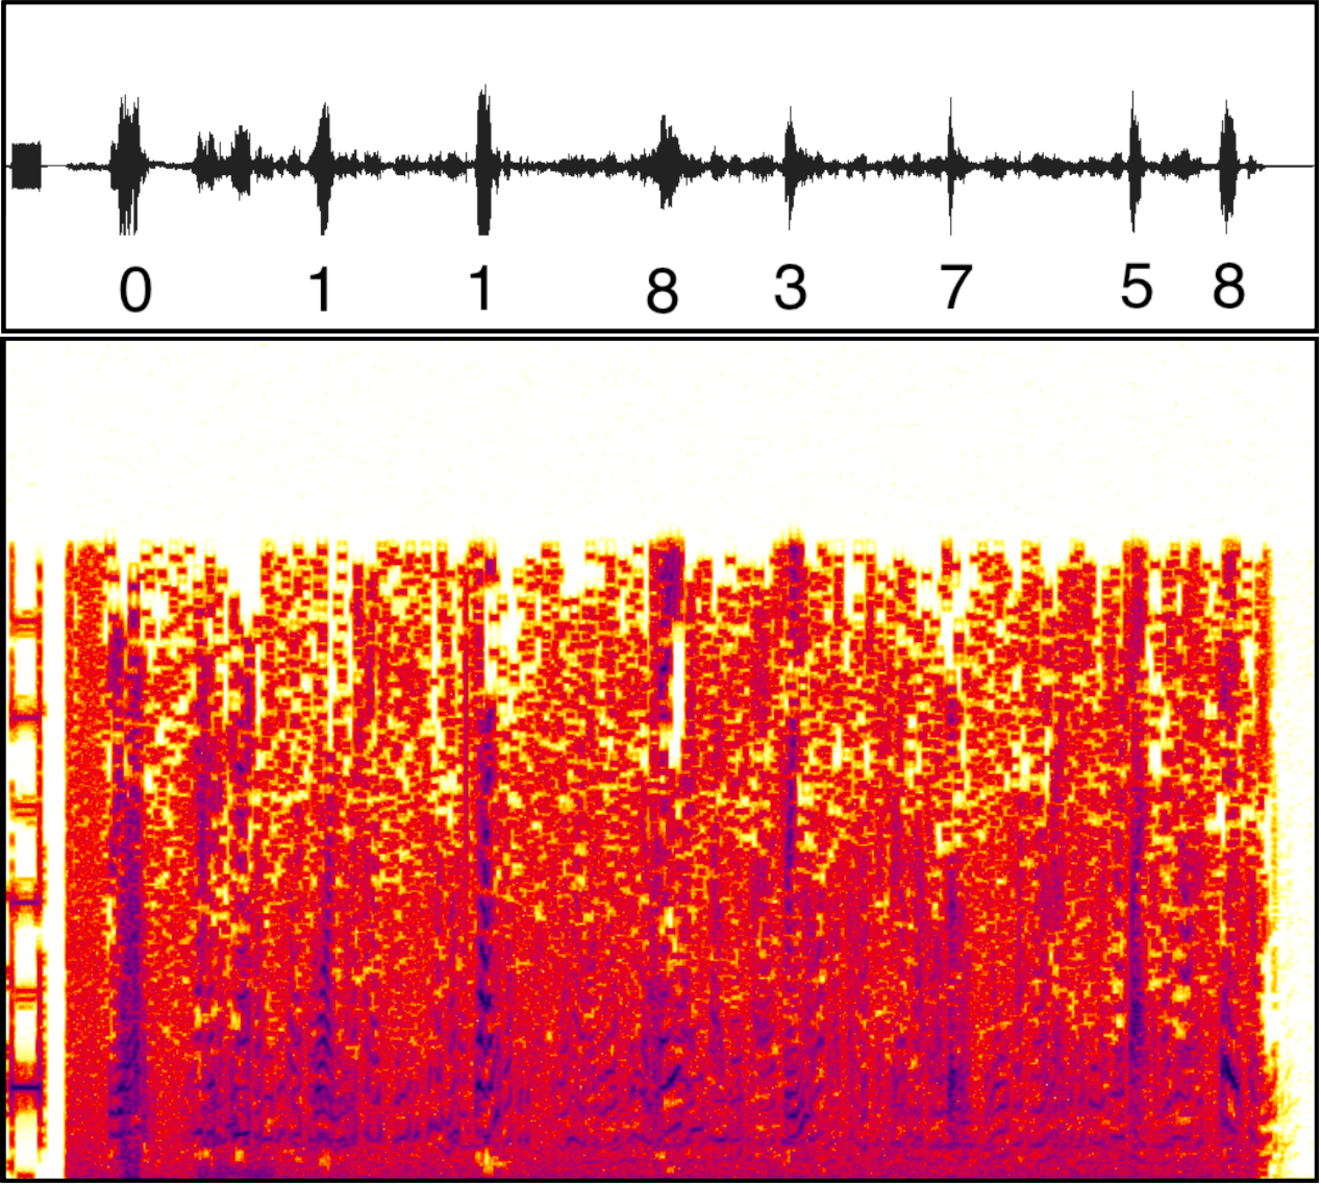
\includegraphics[width=\textwidth]{figures/recaptcha_evolution/2011.pdf}
\caption{\re cca. 2011}
\label{fig:apple}
\end{subfigure} \hspace{0.01\textwidth}
\begin{subfigure}{0.24\textwidth}
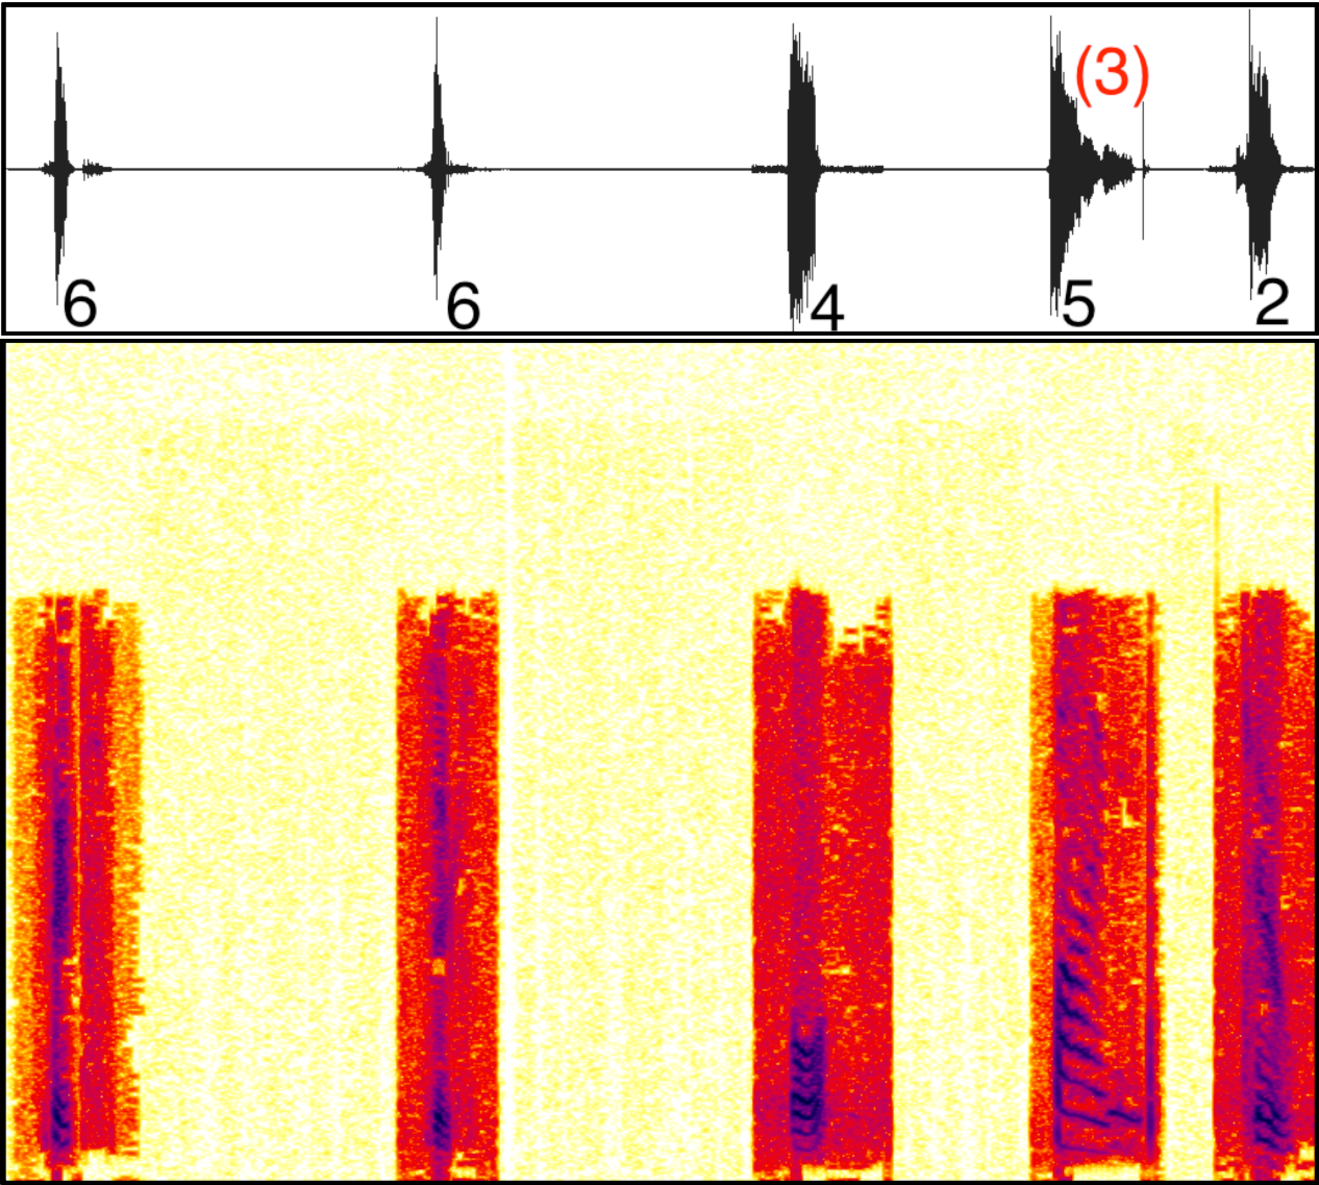
\includegraphics[width=\textwidth]{figures/recaptcha_evolution/2014b.pdf}
\caption{\re cca. 2014}
\label{fig:botdetect}
\end{subfigure}\hspace{0.01\textwidth}
\begin{subfigure}{0.24\textwidth}
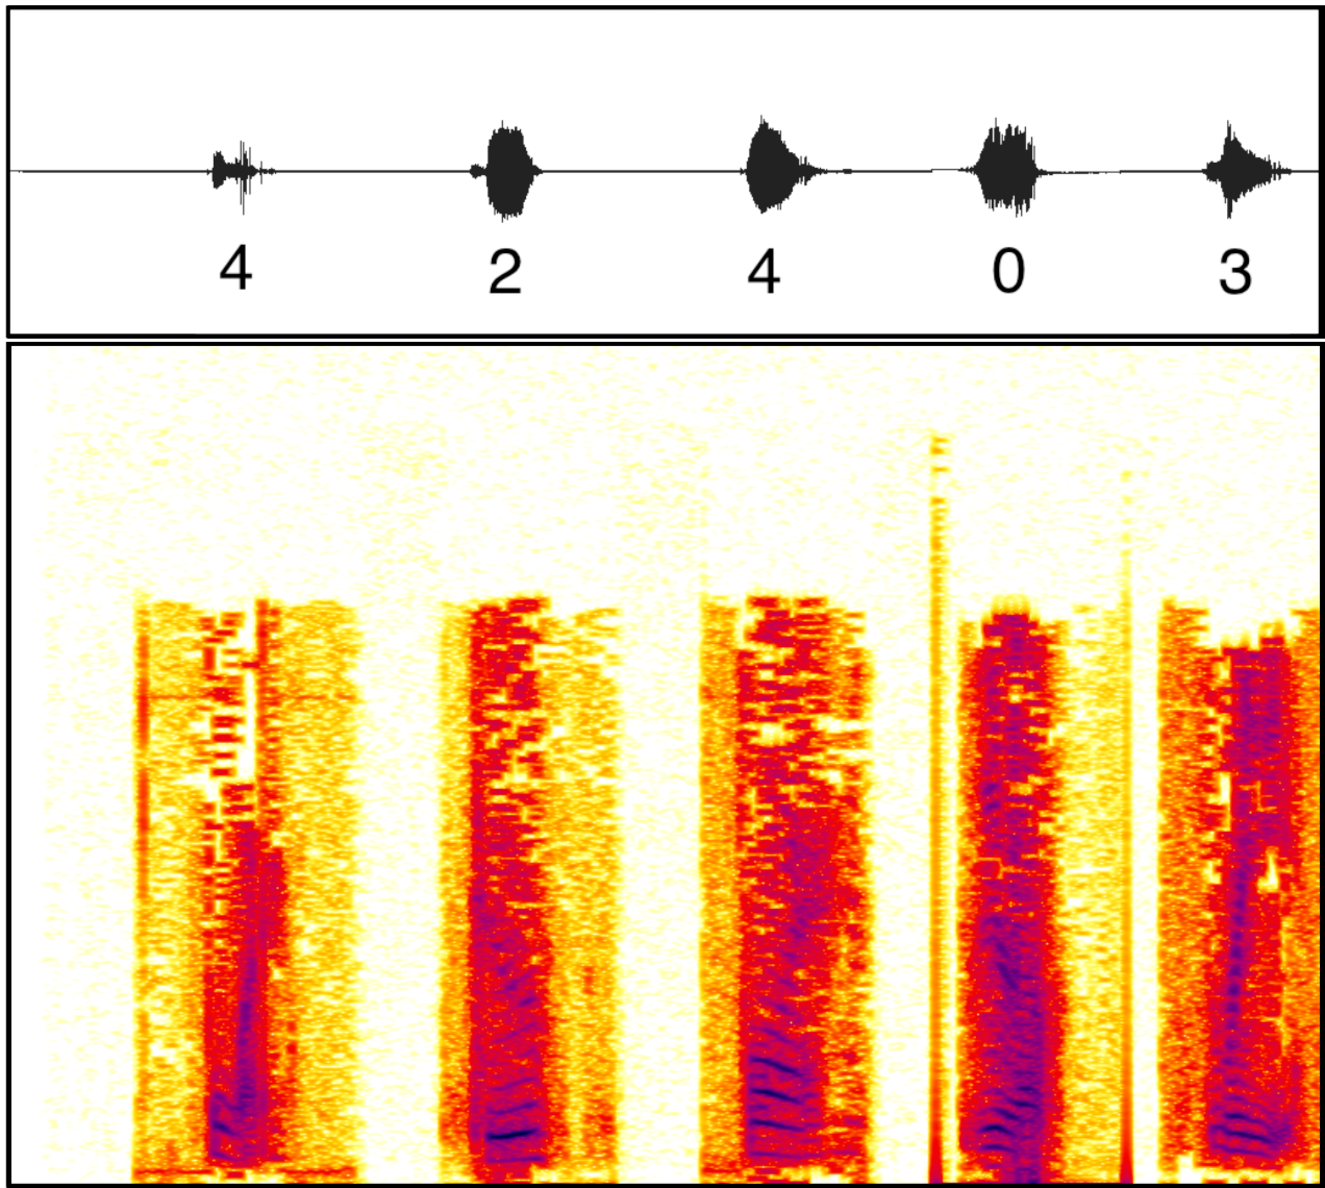
\includegraphics[width=\textwidth]{figures/recaptcha_evolution/2016.pdf}
\caption{\re cca. 2015-2016}
\label{fig:captchas}
\end{subfigure}
\begin{subfigure}{0.24\textwidth}
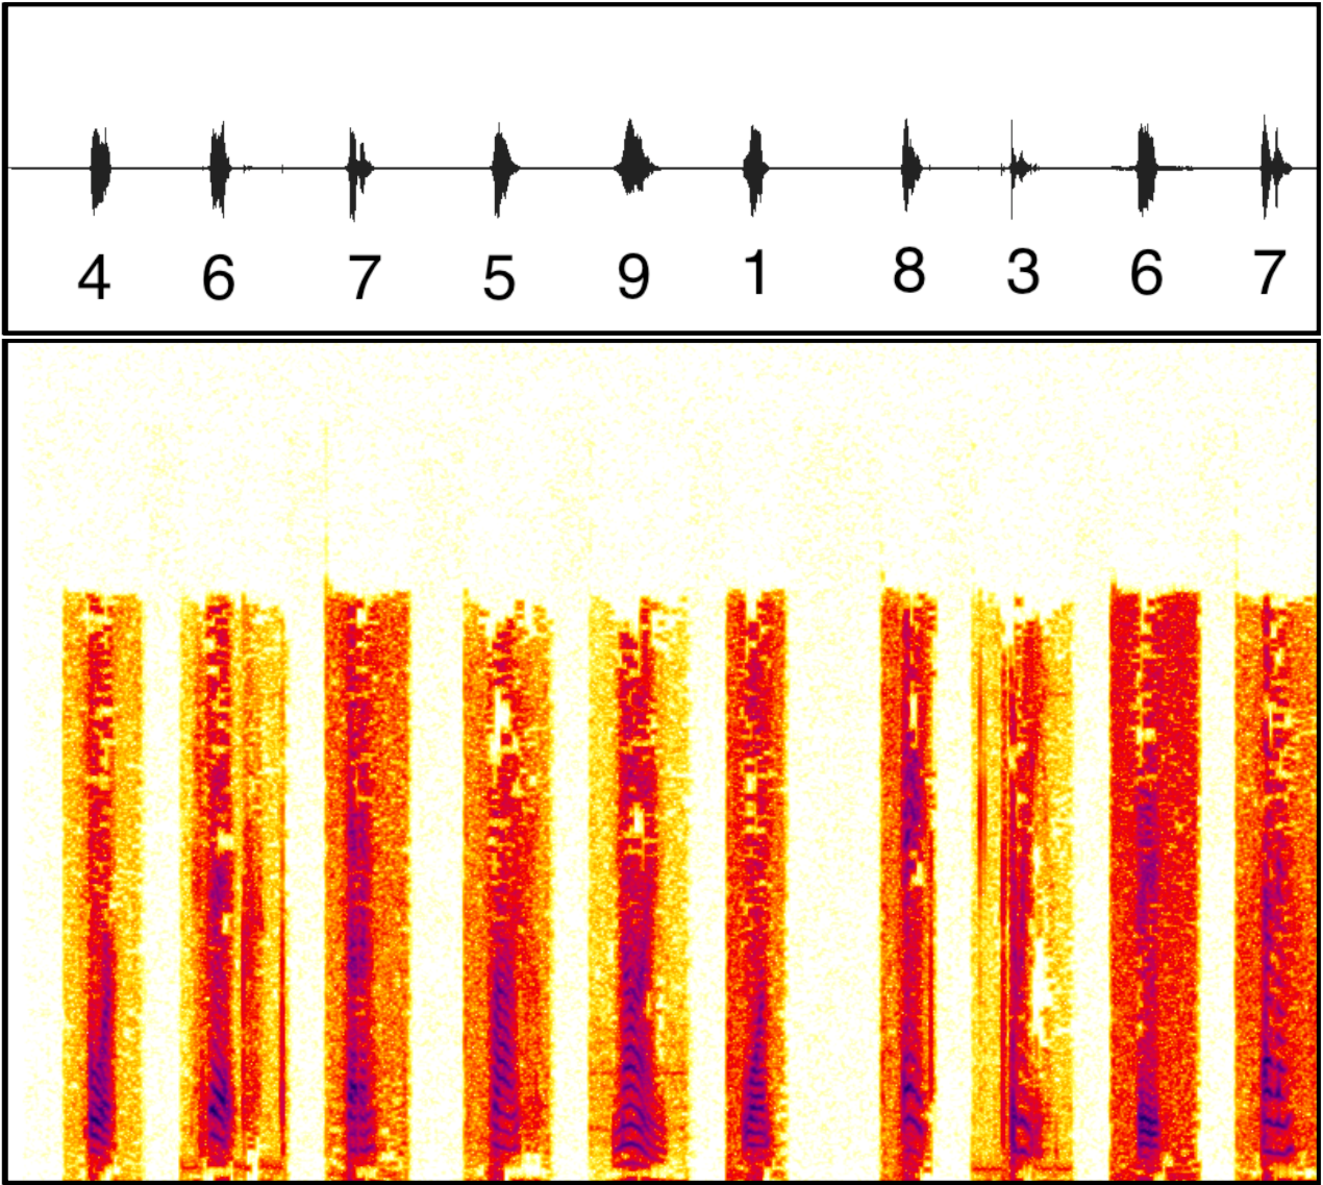
\includegraphics[width=\textwidth]{figures/recaptcha_evolution/2017.pdf}
\caption{\re after March 2017}
\label{fig:live}
\end{subfigure}
\caption{The evolution of \re audio challenges through time.}
\label{fig:evolution}
\end{figure*}


\emph{Evolution through time.} In their extensive user study on the usability of captchas, Burzstein et al.~\cite{captchas-are-hard}
found that users were able to solve only 47\% of \re's audio challenges (that number was calculated following an optimistic approach
and is an upper bound to the actual accuracy). Since then \re has modified their audio challenges. % to be more user friendly.
Here we further explore how audio \re has evolved through time. 

In Figure~\ref{fig:evolution} we visualize audio captcha samples
that capture \re's evolution through time. Indeed, the audio challenges from 2011 are the least ``user-friendly'' as they contain
a significant amount of background noise in the form of unintelligible discussions, reversed recordings of speech. While the version
from 2014 is considerably clearer and only five digits long, the audio quality of the spoken digits remains ``noisy'', while background recordings were
also sporadically interjected. In the sample plotted here, a background recording uttering ``three'' is almost overlapping with the
digit spoken as part of the challenge (shown in red). As part of their ``No Captcha Recaptcha'' system released in December 2014, the audio challenges were 
more simplified as they contained five digits with less noise in the recordings; however, certain recordings are processed and the sounds
are more drawn out. This could potentially be a countermeasure against automated attacks. 
Finally, in the current version which was released in March 2017,
the challenges once again contain 10 digits. 

While there might have been more intermediary changes apart from the ones presented here,
this samples show a clear evolution of audio \re challenges towards a more user-friendly scheme. The change in the latest version 
is most likely an attempt to mitigate automated attacks; however, this can only serve as a temporary measure as our experiments
demonstrate that speech recognition technology has reached a point where such challenges can be trivially bypassed. Thus, it remains 
to be seen whether \re adopts an approach similar to services like Securimage and BotDetect and reverts back to challenges with 
more noise and distortion to hinder automated attacks.

\section{Discussion}
\label{sec:discussion}

While text-based captchas have been the most common type of challenge for years, they have been rendered
obsolete by the demonstration of generic solvers that do not require specific training per captcha system~\cite{185128}.
Recently, researchers demonstrated how deep learning neural networks can be leveraged for breaking image-based 
semantic captchas~\cite{sivakorn:eurosp16}. Our work highlights the ineffectiveness of audio captchas, as 
existing speech recognition systems can be readily applied to transcribing the audio challenges.
As such, it is crucial to design alternative methods for preventing automated attacks; while researchers 
have also considered cognitive games as promising alternatives, they have been found to be vulnerable to 
attacks~\cite{mohamed2017security}.

While prior work has typically explored how additional noise can prohibit automated attacks, these are 
short-lived approaches as machine learning technologies continue to improve and evolve at a radical rate.
Furthemore, audio captchas present an interesting dilemma from a design standpoint, as they are an considerable 
constrained in regards to the ``security versus usability'' tradeoff. Generally, adding more noise (or distortion) 
to combat automated solvers can have a severely negative effect on the ability of users to actually solve challenges.
In the case of audio captchas, this constraint is more pronounced, as human hearing is more error prone than 
vision~\cite{o2009auditory,shinn2008object}.

When taking into consideration that prior work has found popular audio captchas to be much more difficult 
than their visual counterparts~\cite{bigham2009evaluating}, which was also corroborated by a subsequent 
systematic evaluation of users' ability to solve various types of captchas~\cite{captchas-are-hard}, further
distorting existing audio captchas would further hinder visually impaired users from accessing the Web.
Thus, while designing a robust captcha scheme remains an open problem, it is important 
to explore designs that do not present obstacles to certain groups of users (e.g., the visually impaired). 
While this may prove to be an insurmountable constraint, we argue that the current approach of offering audio
challenges is \note{misguided} as they remain an obstacle to visually impaired users while offering 
adversaries a pathway to more accurate attacks.

\section{Related Work}
\label{sec:related}

\textbf{Breaking audio captchas.} Tam et al.~\cite{tam2008improving} were the 
first to evaluate the robustness of audio captchas against automated attacks,
and reported a success rate of 58\% against audio captchas that contained 
digits and random speech segments as background noise. Subsequently, 
Burzstein and Bethard presented Decaptcha, a system that was able to solve 75\%
of eBay's audio captchas~\cite{Bursztein2009}. While they experimented with Sphynx,
which was at the time a state-of-the-art speech recognizer, they were only able to 
achieve a 1\% accuracy. On the other hand, our experiments reveal how speech recognition
technology has greatly evolved, allowing us to solve \note{X-Y\%} of audio challenges
across a large number of services.

Bursztein et al.~\cite{bursztein2011failure} conducted an extensive study on audio audio 
challenges that contained digits and letters and broke the Yahoo, Microsoft, and eBay 
captchas with approximate success rates of 45\%, 49\%, and 83\% respectively. However, 
their system was only able to solve $\sim1.5\%$ of \re challenges, due to the presence 
of semantic noise. More recently, Sano et al.~\cite{Sano2013} focused on the \re
version that contained semantic noise and implemented a custom solver that achieved the best
results up to that point, with a 52\% accuracy. Meutzner et al.~\cite{meutzner2014using} demonstrated 
an improvement over those results and reported a 63\% accuracy against the same version of \re. While
we experiment with the latest versions of \re, which appear to have minor differences, 
we obtain significantly better results with a \note{x\%} accuracy.

\textbf{Captchas and accessibility.} According to Shirali-Shahreza et al.~\cite{shirali2011accessibility},
three groups of people have trouble with visual challenges; the visually impaired,
with dyslexia, and users suffering from motor impairment diseases like Parkinson's.
Chellapilla et al.~\cite{Chellapilla} argued that Human-friendly Interaction Proofs (HIPs)
must approach a success rate of at least 90\%. They also argued that, due to their scale, automated attacks
should be able to solve a challenge in less than 0.01\% of their attempts, for a captcha system to be considered
robust. Sauer et al. conducted a usability study with six blind participants on Google's \re, 
and found that they were only able to solve 46\% of the audio challenges~\cite{sauer2008towards}.
They also found that the average amount of time taken to correctly solve an audio challenge was over 65 seconds.
This is significantly higher than the 28.4 seconds that users required for solving audio captchas
in the extensive user study conducted by Bursztein et al.~\cite{captchas-are-hard}.

While conducting a study with blind high school students, Bigham et al.~\cite{bigham2008inspiring}
found that when the students were presented with an audio captcha, none of them were able to solve the challenge 
and their sighted instructors ended up solving the visual version instead. In a subsequent
study conducted with 89 blind users~\cite{bigham2009evaluating}, they found that users achieved 
only a 43\% success rate when solving 10 popular audio captchas.
%In the same study \cite{bigham2009evaluating}, it was also found that screen readers used by blind users speak over
%playing captchas. As users navigate to the answer box, the accessibility software continue speaking the interface while
%talking over the playing audio challenge. A playing audio challenge does not pause for solvers as they type their answer
%and reviewing an audio captcha is cumbersome, often requiring the user to start again from the beginning. Also, replaying
%an audio captcha requires solvers to navigate away from the answer box in order to access the controls of the audio player.
%Thus, the authors proposed a system and optimized the interface of popular audio captcha services without altering the
%underlying implementation and found that the performance increased to 59\%. 

Holman et al.~\cite{holman2007developing} proposed the extension of image captchas to include related
sounds (e.g., an image challenge showing a train would be accompanied by an audio recording of a train), 
as an alternative type of challenge for blind users. An alternative design that required users to identify 
a series of sounds was later proposed~\cite{Lazar:2012}, and the authors conducted a user study in which the
participants achieved a success rate of over 90\%. Krol et al.~\cite{krol2016better} conducted a user study 
to explore a replacement to current captcha schemes but found that users were apprehensive due to the privacy 
concerns as well as an increased sense of frustration.

\textbf{Applications of audio captchas.} Polakis et al.~\cite{polakis:syssec11} proposed the deployment of 
simple audio challenges (e.g., solving simple math equations, or spelling words with a traditional telephone keypad)
as a defense against automated attacks in telephony systems. Markkola and Lindqvist~\cite{markkola2008accessible}
proposed the deployment of audio captchas that contained digits for preventing telephone SPAM~\cite{sok-robocalls}.

\textbf{Google \re.} In a recent study, Sivakorn et al.~\cite{sivakorn:eurosp16} demonstrated how off-the-shelf 
deep learning systems could be employed for breaking Google's image-based \re system. They also presented a series 
of safeguards employed by \re for preventing automated attacks. Similarly, in our study we demonstrate how off-the-shelf 
speech recognition systems can be used for breaking a wide range of audio captcha systems, and identify a varying set
of safeguards across each captcha service. Interestingly, our experiments demonstrate a significantly higher success rate,
underlining the importance of finding suitable alternatives for accessible captchas, as the availability of audio captchas 
exposes services to significant risks.

\section{Conclusions}
\label{sec:conclusions}

Motivated by the recent advances in speech recognition engines 
built with deep learning neural networks, we conducted a comprehensive 
analysis of the existing audio captcha ecosystem. We demonstrated low-cost attacks that misuse
widely available speech recognition APIs for deploying fully automated attacks
against \no popular captcha schemes. Our extensive experimental evaluation
highlighted the ineffectiveness of existing audio challenges, as all captcha
schemes were broken by our \system system. Among other surprising results,
we found that \re, the most prevalent captcha service, is among the most 
trivial challenges to pass  Furthermore, \re audio challenges facilitate 
fraudsters, as they are are susceptible to significantly more accurate attacks
than their visual counterparts. Given the physical limitations of human hearing
in the presence of auditory noise, reconciling the opposing notions of security 
and usability in the era of deep learning is a daunting task. In their current form,
audio captchas remain obstacles for certain users and fail to offer adequate security.
Thus, it is of paramount importance to explore new directions for ensuring accessibility
for all users while preventing automated attacks.




\bibliographystyle{ACM-Reference-Format}
\bibliography{paper}

\end{document}
